\documentclass[12pt]{article}
\usepackage{amsfonts}
\usepackage{listings}
\usepackage{amsmath}
\usepackage{amsthm}
\usepackage{algorithmicx}
\usepackage{algpseudocode}
\usepackage{graphicx}
\usepackage{tikz}
\usepackage{float}
\pagestyle{myheadings}
\usepackage{verbatim}
%\widowpenalties 1 10000

\author{Peter Ahrens, Hong Diep Nguyen, James Demmel}
\title{ReproBLAS: Much Summation! So Reproducible!}
\providecommand{\R}{\ensuremath{\mathbb{R}}}
\providecommand{\F}{\ensuremath{\mathbb{F}}}
\providecommand{\Z}{\ensuremath{\mathbb{Z}}}
\providecommand{\exp}{\ensuremath{\text{exp}}}
\providecommand{\min}{\ensuremath{\text{min}}}
\providecommand{\max}{\ensuremath{\text{max}}}
\providecommand{\ulp}{\ensuremath{\text{ulp}}}
\providecommand{\ufp}{\ensuremath{\text{ufp}}}
\providecommand{\fl}{\ensuremath{\text{fl}}}
\providecommand{\To}{\ensuremath{\text{ to }}}
\providecommand{\roundtonearestinfty}{\ensuremath{\mathcal{R}_\text{$\infty$}}}
\theoremstyle{definition}
\newtheorem{thm}{Theorem}[section]
\newtheorem{lem}[thm]{Lemma}
\newtheorem{alg}{Algorithm}[section]
\numberwithin{equation}{section}
\numberwithin{figure}{section}

\graphicspath{{plots}}
\begin{document}
\noindent
\maketitle
\tableofcontents
\newpage
\section{Introduction}
\section{Notation and Background}
  Let $\R, \F, $ and $\Z$ denote the sets of real numbers, floating-point numbers, and integers respectively.

  For all $r \in \R$, let $r\Z$ denote the set of all multiples of $r$, $\{rz | z \in \Z\}$.

  For all $r \in \R$, let $\lfloor r \rfloor$ be the minimum element $z \in \Z$ such that $z \geq r$.

  For all $r \in \R$, let $\lceil r \rceil$ be the maximum element $z \in \Z$ such that $z \leq r$.

  We define the function $\roundtonearestinfty(r, e), r \in R, e \in \Z$ as

  \begin{equation}
    \roundtonearestinfty(r, e) = \begin{cases}\lfloor r/2^e + 1/2 \rfloor 2^e \text{ if } r \geq 0\\ \\ \lceil r/2^e - 1/2 \rceil 2^e \text{ otherwise}\end{cases}
  \end{equation}

  $\roundtonearestinfty(r, e)$ rounds $r$ to the nearest multiple of $2^e$, breaking ties away from 0. A property of such rounding is shown in  \eqref{eq:round}

  \begin{equation}
    \bigl|r - \roundtonearestinfty(r, e)\bigr| \leq 2^{e - 1}
    \label{eq:round}
  \end{equation}

  Assume that floating point arithmetic complies with the IEEE 754-2008 standard \cite{ieee754} in some ``to nearest'' rounding mode (no specific tie breaking behaviour is required) and that underflow occurs gradually, although methods to handle abrupt underflow will be considered in Section \ref{sec:indexed_underflow_abrupt}.

  Let $f = sm2^e \in \F$ be a floating-point number represented in IEEE 754-2008 format \cite{ieee754} where $s \in \{1, -1\}$ is the \textbf{sign}, $e_{\max} \geq e \geq e_{\min}$ is the \textbf{exponent} ($\exp(f)$ is defined to be $e$), $p$ is the \textbf{precision}, and $m = m_0.m_1m_2...m_{p-1}$ where $m_0, ..., m_{p - 1} \in \{0, 1\}$ is the \textbf{significand} of $f$. $f$ is said to be \textbf{normalized} if $m_0 = 1$ and $e \geq e_{\min}$, \textbf{unnormalized} if $m_0 = 0$, and \textbf{denormalized} if $m_0 = 0$ and $e = e_{\min}$. $f = 0$ if all $m_k = 0$ and $e = e_{\min}$.

  $r \in \R$ is \textbf{representable} as a floating point number if there exists $f \in \F$ such that $r = f$ as real numbers.

  For all $r \in \R$, $e \in \Z$ such that $e_{\min} - p < e$ and $|r| < 2 \cdot 2^{e_{\max}}$, if $r \in 2^e\Z$ and $r \leq 2^{e + p}$ then $r$ is representable.

  Machine epsilon, $\epsilon$, the difference between 1 and the greatest floating point number smaller than 1, is defined as $\epsilon = 2^{-p}$.

  The unit in the last place of $f \in \F$, $\ulp(f)$, is the spacing between two consecutive floating point numbers of the same exponent as $f$. If $f$ is normalized, $\ulp(f) = 2^{\exp(f) - p + 1} = 2  \epsilon  2^{\exp(f)}$ and $\ulp(f) < 2^{p - 1}|f|$.

  The unit in the first place of $f \in F$, $\ufp(f)$, is the value of the first significant bit of $f$. If $f$ is normalized, $\ufp(f) = 2^{\exp(f)}$.

  For all $f_0, f_1 \in \F$, $\fl(f_0 \text{ op } f_1)$ denotes the evaluated result of the expression $(f_0 \text{ op } f_1)$ in floating point arithmetic. If $(f_0 \text{ op } f_1)$ is representable, then $\fl(f_0 \text{ op } f_1) = (f_0 \text{ op } f_1)$. If rounding is ``to nearest,'' then we have that $|\fl(f_0 \text{ op } f_1) - (f_0 \text{ op } f_1)| \leq \frac{1}{2}\ulp(\fl(f_0 \text{ op } f_1))$.

  As ReproBLAS is written in C, \texttt{float} and \texttt{double} refer to the floating point types specified in the 1989 C standard \cite{c89} and we assume that they correspond to the \texttt{binary-32} and \texttt{binary-64} types in the IEEE 754-2008 floating point standard \cite{ieee754}.

  All indices start at $0$ in correspondence with the actual ReproBLAS implementation.
\section{Binning}
  \label{sec:binning}
    We achieve reproducible summation of floating point numbers through binning. Each number is split into several components corresponding to predefined ranges, then the components corresponding to each range are accumulated separately. We begin in Section \ref{sec:binning_bins} by explaining the particular set of ranges (referred to as bins) used. Section \ref{sec:binning_slices} develops original mathematical theory to describe the components (referred to as slices) corresponding to each range. We develop this theory to concisely describe and prove correctness of algorithms throughout the paper (especially Algorithms \ref{alg:depositrestricted} and \ref{alg:deposit}).
  \subsection{Bins}
    \label{sec:binning_bins}
    We start by dividing the exponent range $(e_{\min} - p, ..., e_{\max} + 1]$  into \textbf{bins} $(a_i, b_i]$ of \textbf{width} $W$ according to \eqref{eq:imax}, \eqref{eq:a}, and \eqref{eq:b}. Such a range is used so that the largest and smallest (denormalized) floating point numbers may be approximated.

    \begin{equation}
      i_{\max} = \bigl\lfloor(e_{\max} - e_{\min} + p - 1)/W\bigr\rfloor - 1
      \label{eq:imax}
    \end{equation}

    \begin{equation}
      a_i = e_{\max} + 1 - (i + 1)W,\; 0 \leq i \leq i_{\max}
      \label{eq:a}
    \end{equation}

    \begin{equation}
      b_i = a_i + W
      \label{eq:b}
    \end{equation}

    We say the bin $(a_{i_0}, b_{i_0}]$ is \textbf{greater} than the bin $(a_{i_1}, b_{i_1}]$ if $a_{i_0} > a_{i_1}$ (which is equivalent to both $b_{i_0} > b_{i_1}$ and $i_0 < i_1$).

    We say the bin $(a_{i_0}, b_{i_0}]$ is \textbf{lesser} than the bin $(a_{i_1}, b_{i_1}]$ if $a_{i_0} < a_{i_1}$ (which is equivalent to both $b_{i_0} < b_{i_1}$ and $i_0 > i_1$).

    We use $i \leq i_{\max} = \lfloor(e_{\max} - e_{\min} + p - 1)/W\rfloor - 1$ to ensure that $a_i > e_{\min} - p + 1$ as discussed in Section \ref{sec:indexed_underflow_gradual}. This means that the greatest bin, $(a_{0}, b_{0}]$, is

    \begin{equation}
      (e_{\max} + 1 - W, e_{\max} + 1]
      \label{eq:binmax}
    \end{equation}

    and the least bin, $(a_{i_{\max}}, b_{i_{\max}}]$, is

    \begin{equation}
      \Bigl(e_{\min} - p + 2 + \bigl((e_{\max} - e_{\min} + p - 1)\mod W\bigr),
      e_{\min} - p + 2 + W + \bigl((e_{\max} - e_{\min} + p - 1)\mod W\bigr)\Bigr]
      \label{eq:binmin}
    \end{equation}

    Section \ref{sec:indexed_underflow_gradual} explains why the range

    \begin{equation*}
    \Bigl(e_{\min} - p, e_{\min} - p + 2 + \bigl((e_{\max} - e_{\min} + p - 1) \mod W\bigr)\Bigr]
    \end{equation*}

    is ignored.

    As discussed in \cite{repsum}, we must assume
    \begin{equation}
      W < p - 2
      \label{eq:wupper}
    \end{equation}

    As discussed in Section \ref{sec:indexed_overflow}, we must also assume
    \begin{equation}
      2 W > p + 1
      \label{eq:wlower}
    \end{equation}

    ReproBLAS uses both \texttt{float} and \texttt{double} floating point types. The chosen division of exponent ranges for both types is shown in Figure \ref{fig:bins}.
    \begin{figure}[H] \centering\begin{tabular}{ | l | l | l | p{5cm} |} \hline Floating-Point Type & \texttt{float} & \texttt{double}\\ \hline $e_{\max}$ & 127 & 1023\\ \hline $e_{\min}$ &  -126 & -1022 \\ \hline $p$ & 24 & 53 \\ \hline $e_{\min} - p$ & -140 & -1075 \\ \hline $W$ & 13 & 40 \\ \hline $i_{\max}$ & 19 & 51 \\ \hline $(a_0, b_0]$ & $(115, 128]$ & $(984, 1024]$\\ \hline $(a_{i_{\max}}, b_{i_{\max}}]$ & $(-132, -119]$ & $(-1056, -1016]$ \\ \hline\end{tabular} \caption{ReproBLAS Binning Scheme}\label{fig:bins}\end{figure}

  \subsection{Slices}
    \label{sec:binning_slices}
    Throughout the text we will refer to the \textbf{slice} of some $x \in \F$ in the bin $(a_i, b_i]$. $x$ can be split into several slices, each slice corresponding to a bin $(a_i, b_i]$ and expressible as the (possibly negated) sum of a subset of $\{2^e, e \in (a_i, b_i]\}$, such that the sum of the slices provides a good approximation of $x$. Specifically, the slice of $x \in \F$ in the bin $(a_i, b_i]$ is defined recursively as $d(x, i)$ in \eqref{eq:d}. We must define $d(x, i)$ recursively because it is not a simple bitwise extraction.
    \begin{equation}
      d(x, i) = \roundtonearestinfty\bigl(x - \sum\limits_{k=0}^{i - 1}d(x,k), a_i + 1\bigr)
      \label{eq:d}
    \end{equation}

    We make three initial observations on the definition of $d(x, i)$. First, we note that $d(x, i)$ is well defined recursively on $i$ with base case $d(x, 0) = \roundtonearestinfty(x, a_0 + 1)$.

    Next, notice that $d(x, i) \in 2^{a_{i} + 1}\Z$.

    Finally, it is possible that $d(x, 0)$ may be too large to represent as a floating point number. Overflow of this type is accounted for in Section \ref{sec:indexed_overflow}.

    Lemmas \ref{lem:dzero} and \ref{lem:dmiddle} follow from the definition of $d(x, i)$.

    \begin{samepage}
    \begin{lem}
      For all $i \in \{0, ..., i_{\max}\}$ and $x \in \F$ such that $|x| < 2^{a_i}$, $d(x, i) = 0$
      \label{lem:dzero}
    \end{lem}
    \end{samepage}

    \begin{proof}
      We show the claim by induction on $i$.

      In the base case, we have $|x| < 2^{a_0}$ and $d(x, 0) = \roundtonearestinfty(x, a_0 + 1)$. By the triangle inequality and  \eqref{eq:round},
      \begin{equation*}
        \bigl|\roundtonearestinfty(x, a_0 + 1)\bigr| \leq |x| + \bigl|x - \roundtonearestinfty(x, a_0 + 1)\bigr| < 2^{a_0 + 1}
      \end{equation*}
      Since $\roundtonearestinfty(x, a_0 + 1) \in 2^{a_0 + 1}\Z$, we then have
      \begin{equation*}
        d(x, 0) = \roundtonearestinfty(x, a_0 + 1) = 0
      \end{equation*}

      In the inductive step, we have $|x| < 2^{a_{i + 1}} \leq ... \leq 2^{a_0}$ by  \eqref{eq:a} and by induction $d(x, i)= ... = d(x, 0) = 0$. Thus,
      \begin{equation*}
        d(x, i + 1) = \roundtonearestinfty\bigl(x - \sum\limits_{k = 0}^{i}d(x, k), a_{i + 1} + 1\bigr) = \roundtonearestinfty(x, a_{i+1} + 1)
      \end{equation*}
      Again by the triangle inequality and  \eqref{eq:round},
      \begin{equation*}
        \bigl|\roundtonearestinfty(x, a_{i + 1} + 1)\bigr| \leq |x| + \bigl|x - \roundtonearestinfty(x, a_{i + 1} + 1)\bigr| < 2^{a_{i + 1} + 1}
      \end{equation*}
      Since $\roundtonearestinfty(x, a_{i + 1} + 1) \in 2^{a_{i + 1} + 1}\Z$, we then have
      \begin{equation*}
        d(x, i + 1) = \roundtonearestinfty(x, a_{i + 1} + 1) = 0
      \end{equation*}
    \end{proof}

    \begin{samepage}
    \begin{lem}
      For all $i \in \{0, ..., i_{\max}\}$ and $x \in \F$ such that $|x| < 2^{b_i}$, $d(x, i) = \roundtonearestinfty(x, a_i + 1)$.
      \label{lem:dmiddle}
    \end{lem}
    \end{samepage}

    \begin{proof}
      The claim is a simple consequence of Lemma \ref{lem:dzero}.

      By  \eqref{eq:a} and \eqref{eq:b}, $|x| < 2^{b_i} = 2^{a_{i - 1}} \leq  ... \leq 2^{a_0}$. Therefore Lemma \ref{lem:dzero} implies $d(x, 0) = ... = d(x, i - 1) = 0$ and we have \begin{equation*}
        d(x, i) = \roundtonearestinfty\bigl(x - \sum\limits_{k = 0}^{i - 1}d(x, k), a_{i} + 1\bigr) = \roundtonearestinfty(x, a_{i} + 1)
      \end{equation*}
    \end{proof}

    Lemma \ref{lem:dzero}, Lemma \ref{lem:dmiddle}, and \eqref{eq:d} can be combined to yield an equivalent definition of $d(x, i)$ for all $i \in \{0, ..., i_{\max}\}$ and $x \in \F$.

    \begin{equation}
      d(x, i) = \begin{cases}0 \text{ if } |x| < 2^{a_i}\\ \roundtonearestinfty(x, a_i + 1) \text{ if } 2^{a_i} \leq |x| < 2^{b_i}\\\roundtonearestinfty\bigl(x - \sum\limits_{k=0}^{i - 1}d(x,k), a_i + 1\bigr) \text{ if } 2^{b_i} \leq |x| \end{cases}
      \label{eq:d2}
    \end{equation}

    Theorem \ref{thm:dround} shows that sum of the slices of $x \in \F$ provides a good approximation of $x$.

    \begin{samepage}
    \begin{thm}
      For all $i \in \{0, ..., i_{\max}\}$ and $x \in \F$, $|x - \sum \limits_{k = 0}^id(x, k)| \leq 2^{a_i}$.
      \label{thm:dround}
    \end{thm}
    \end{samepage}

    \begin{proof}
      We apply  \eqref{eq:round} and \eqref{eq:d2}
      \begin{align*}
        \bigl|x - \sum \limits_{k = 0}^{i}d(x, k)\bigr| & = \Bigl|\bigl(x - \sum \limits_{k = 0}^{i - 1}d(x, k)\bigr) - d(x, i)\Bigr| \\
         & = \Bigl|\bigl(x - \sum \limits_{k = 0}^{i - 1}d(x, k)\bigr) - \roundtonearestinfty\bigl(x - \sum \limits_{k = 0}^{i - 1}d(x, k), a_{i} + 1\bigr)\Bigr| \leq 2^{a_{i}}
      \end{align*}
    \end{proof}

    Theorem \ref{thm:dbound} shows a bound on $d(x, i)$.

    \begin{samepage}
    \begin{thm}
      For all $i \in \{0, ..., i_{\max}\}$ and $x \in \F$, $|d(x, i)| \leq 2^{b_i}$.
      \label{thm:dbound}
    \end{thm}
    \end{samepage}

    \begin{proof}
      First, we show that $|x - \sum\limits_{k=0}^{i - 1}d(x,k)| \leq 2^{b_i}$.

      If $i = 0$, then we have
      \begin{equation*}
        \bigl|x - \sum\limits_{k=0}^{i - 1}d(x,k)\bigr| = |x| < 2 \cdot 2^{e_{\max}} < 2^{b_0}
      \end{equation*}
      Otherwise, we can apply  \eqref{eq:a} and \eqref{eq:b} to Theorem \ref{thm:dround} to get
      \begin{equation*}
        \bigl|x - \sum \limits_{k = 0}^{i - 1}d(x, k)\bigr| \leq 2^{a_{i - 1}} = 2^{b_i}
      \end{equation*}

      As $2^{b_i} \in 2^{a_i + 1}\Z$,  \eqref{eq:d} can be used

      \begin{equation*}
        \bigl|d(x, i)\bigr| = \Bigl|\roundtonearestinfty\bigl(x - \sum\limits_{k=0}^{i - 1}d(x,k), a_i + 1\bigr)\Bigr| \leq 2^{b_i}
      \end{equation*}
    \end{proof}

\section{The Indexed Type}
  \label{sec:indexed}
    The \textbf{indexed type} is used to represent the intermediate result of accumulation using Algorithms 6 and $7$ in \cite{repsum}.
    An indexed type $Y$ is a data structure composed of several accumulator data structures $Y_0, ..., Y_{K - 1}$. An indexed type with $K$ accumulators is referred to as a \textbf{$K$-fold} indexed type. Due to their low accuracy, 1-fold indexed types are not considered.

    Let $Y$ be the indexed type corresponding to the reproducibly computed sum of $x_0, ..., x_{n - 1} \in \F$.
    Each accumulator $Y_j$ is a data structure used to accumulate the slices of input in the bin $(a_{I + j}, b_{I + j}]$ where $I$ is the \textbf{index} of $Y$ and $j \geq 0$ as discussed below. The \textbf{width} of an indexed type is equal to the width of its bins, $W$. Recall the assumptions \eqref{eq:wupper} and \eqref{eq:wlower} made on the value of $W$.

    The accumulators in an indexed type correspond to contiguous bins in decreasing order. The index of $Y$ is defined as the least $I \in \Z$ such that $2^{b_I + 1} > \max(|x_0|, ..., |x_n|)$ (equivalently, the least $I \in \Z$ such that $b_I > \max(e_0, ..., e_n)$). If $Y$ has index $I$, then $Y_j, j \in \{0, ..., K - 1\}$ accumulates slices of input in the bin $(a_{I + j}, b_{I + j}]$. If $I$ is so large that $I + K > i_{\max}$, then the extra $I + K - i_{\min}$ accumulators are unused.

    Section \ref{sec:indexed_primary_carry} elaborates on the specific fields that make up the indexed type and the values they represent. Sections \ref{sec:indexed_overflow}, \ref{sec:indexed_underflow_gradual}, \ref{sec:indexed_underflow_abrupt}, and \ref{sec:indexed_exceptions} contain original extensions of the indexed type to handle overflow, underflow, and exceptional values.

    \subsection{Primary and Carry}
      \label{sec:indexed_primary_carry}
      As discussed in \cite{repsum}, indexed types are represented using floating point numbers to minimize traffic between floating point and integer arithmetic units.

      In the ReproBLAS library, if an indexed type is used to sum \texttt{doubles}, then it is composed entirely of \texttt{doubles} and likewise for \texttt{floats}. ReproBLAS supports complex types as pairs of real and imaginary components (stored contiguously in memory). If an indexed type is used to sum complex \texttt{doubles} or \texttt{floats}, then it is composed of pairs (real part, imaginary part) of \texttt{doubles} or \texttt{floats} respectively. The decision to keep the real and imaginary components together (as opposed to keeping separate indexed types for real and imaginary parts of the sum) was motivated by a desire to process accumulators simultaneously with vectorized (SIMD) instructions.

      The accumulators $Y_j$ of an indexed type $Y$ are each implemented using two underlying floating point fields. The \textbf{primary} field ${Y_j}_P$ is used during accumulation, while the \textbf{carry} field ${Y_j}_C$ holds overflow from the primary field. Because primary fields are frequently accessed sequentially, the primary fields and carry fields are each stored contiguously in separate arrays. The notation for the primary field ${Y_j}_P$ and carry field ${Y_j}_C$ corresponds to the ``$S_k$'' and ``$C_k$'' of Algorithm $6$ in \cite{repsum}.

      The numerical value ${\mathcal{Y}_j}_P$ represented by data stored in the primary field ${Y_j}_P$ is an offset from $1.5\epsilon^{-1}2^{a_{I + j}}$ (corresponding to ``$M_{[i]}$'' at the beginning of Section IV.A. in \cite{repsum}), where $I$ is the index of $Y$, as shown in  \eqref{eq:pri} below.
      \begin{equation}
        {\mathcal{Y}_j}_P = {Y_j}_P - 1.5\epsilon^{-1}2^{a_{I + j}}
        \label{eq:pri}
      \end{equation}
      This simplifies the process of extracting the slices of input in bins $(a_{I + j}, b_{I + j}]$. It will be shown in Theorem \ref{thm:ddepositrestricted} that if we represent each primary value ${\mathcal{Y}_j}_P$ as in \eqref{eq:pri} and keep ${Y_j}_P$ within the range $(\epsilon^{-1} 2^{a_{I + j}}, 2 \epsilon^{-1} 2^{a_{I + j}})$, then Algorithm \ref{alg:depositrestricted} extracts the slices of $x$ in bins $(a_I, b_I], ..., (a_{I + K - 1}, b_{I + K - 1}]$ and adds them to ${Y_0}_P, ..., {Y_{K - 1}}_P$ without error (and hence reproducibly) for all $x \in \F$, where $|x| < 2^{b_I}$.

      Because $d(x, I + j) = 0$ for bins with $x < 2^{a_{I + j}}$, the values in the greatest $K$ nonzero accumulators can be computed reproducibly by computing the values in the greatest $K$ accumulators needed for the largest $x$ seen so far. Upon encountering an $x \geq 2^{b_I}$, the accumulators can then be shifted towards index $0$ as necessary. \cite{repsum} contains further discussions of the reproducibility of the algorithm.

      In order to keep the primary fields in the necessary range while the slices are accumulated and to keep the representation of $Y_j$ unique, ${Y_j}_P$ is routinely renormalized to the range $[1.5 \epsilon^{-1} 2^{a_{I + j}}, 1.75 \epsilon^{-1} 2^{a_{I + j}})$. Section \ref{sec:primitiveops_renormalize} contains a discussion of how often such renormalizations are necessary.
      To renormalize, ${Y_j}_P$ is incremented or decremented by $0.25 \epsilon^{-1} 2^{a_{I + j}}$ when necessary, leaving the carry field ${Y_j}_C$ to record the number of such adjustments.
      The numerical value ${\mathcal{Y}_j}_C$ represented by data stored in the carry field ${Y_j}_C$ of an indexed type $Y$ of index $I$ is expressed in \eqref{eq:car}
      \begin{equation}
        {\mathcal{Y}_j}_C = (0.25\epsilon^{-1}2^{a_{I + j}}){Y_j}_C
        \label{eq:car}
      \end{equation}
      Combining \eqref{eq:pri} and \eqref{eq:car}, we get that the value $\mathcal{Y}_j$ of the accumulator $Y_j$ of an indexed type $Y$ of index $I$ is
      \begin{equation}
        \mathcal{Y}_j = {\mathcal{Y}_j}_P + {\mathcal{Y}_j}_C = ({Y_j}_P - 1.5 \epsilon^{-1}2^{a_{I + j}}) + (0.25\epsilon^{-1}2^{a_{I + j}}){Y_j}_C
        \label{eq:acc}
      \end{equation}
      Therefore, using  \eqref{eq:acc}, the numerical value $\mathcal{Y}$ represented by data stored in a $K$-fold indexed type $Y$ of index $I$ (the sum of $Y$'s accumulators) is
      \begin{equation}
        \mathcal{Y} = \sum\limits_{j = 0}^{K - 1} \mathcal{Y}_j = \sum\limits_{j = 0}^{K - 1} \bigl(({Y_j}_P - 1.5 \epsilon^{-1}2^{a_{I + j}}) + (0.25\epsilon^{-1}2^{a_{I + j}}){Y_j}_C\bigr)
        \label{eq:indexedvalue}
      \end{equation}
      It is worth noting here that because the primary field ${Y_0}_P$ is stored with an exponent of $a_I + p$, it is unnecessary to store the index of an indexed type explicitly. The index can be determined by simply examining the exponent of ${Y_0}_P$, as all $a_I$ are distinct and the mapping between the exponent of ${Y_0}_P$ and the index of $Y$ is bijective.

    \subsubsection{Overflow}
      \label{sec:indexed_overflow}
      If an indexed type $Y$ has index 0 and the width is $W$, then the value in the primary field ${Y_0}_P$ is stored as an offset from $1.5\epsilon^{-1}2^{e_{\max} + 1 - W}$. However, $1.5\epsilon^{-1}2^{e_{\max} + 1 - W} > 2^{e_{\max} + 1 + (p - W)} > 2 \cdot 2^{e_{\max}}$ since $W < p - 2$ \cite{repsum}, so it is out of the range of the floating-point system and not representable. Before discussing the solution to this overflow problem, take note of Theorem \ref{thm:overflow}.

      \begin{samepage}
      \begin{thm}
        If $2 W > p + 1$, then for any indexed type $Y$ of index $I$ and any ${Y_j}_P$ such that $I + j \geq 1$, $|{Y_j}_P| < 2^{e_{\max}}$.
        \label{thm:overflow}
      \end{thm}
    \end{samepage}

      \begin{proof}
        $a_1 = e_{\max} + 1 - 2 W$ by definition, therefore $a_1 < e_{\max} - p$ and since all quantities are integers, $a_1 \leq e_{\max} - p - 1$. As $a_0, a_1, ...$ is a positive decreasing sequence, $a_{I + j} \leq e_{\max} - p - 1$ since $I + j \geq 1$.

        ${Y_j}_P$ is kept within the range $(\epsilon^{-1} 2^{a_{I + j}}, 2 \epsilon^{-1} 2^{a_{I + j}})$, therefore
        \begin{equation*}
          |{Y_j}_P| < 2 \epsilon^{-1} 2^{a_{I + j}} \leq 2^{1 + p} 2^{e_{\max} - 1 - p} = 2^{e_{\max}}
        \end{equation*}
      \end{proof}
      By Theorem \ref{thm:overflow}, if $2 W > p + 1$ then the only primary field that could possibly overflow is a primary field corresponding to bin 0, and all other primary fields have exponent less than $e_{\max}$. Therefore, we impose $2 W > p + 1$ and express the value of the primary field corresponding to bin 0 as a scaled offset from $1.5\cdot2^{e_{\max}}$. Note that this preserves uniqueness of the exponent of the primary field corresponding to bin 0 because no other primary field has an exponent of $e_{\max}$. The value ${\mathcal{Y}_0}_P$ stored in the primary field ${Y_0}_P$ of an indexed type $Y$ of index 0 is expressed in \eqref{eq:pri0}.
      \begin{equation}
        {\mathcal{Y}_0}_P = 2^{p - W + 1}({Y_0}_P - 1.5\cdot2^{e_{\max}})
        \label{eq:pri0}
      \end{equation}
    \subsubsection{Gradual Underflow}
      \label{sec:indexed_underflow_gradual}
      Here we consider the effects of gradual underflow on algorithms described in \cite{repsum} and how the indexed type allows these algorithms to work correctly.

      Algorithms \ref{alg:deposit} and \ref{alg:renorm} require that the primary fields ${Y_j}_P$ are normalized to work correctly. Theorem \ref{thm:underflowufp} shows that the primary fields should always be normalized.

      \begin{samepage}
      \begin{thm}
        For any primary field ${Y_j}_P$ of an indexed type $Y$ of index $I$ where ${Y_j}_P \in (\epsilon^{-1} 2^{a_{I + j}}, 2 \epsilon^{-1} 2^{a_{I + j}})$ (${Y_0}_P \in (2^{e_{\max}}, 2 \cdot 2^{e_{\max}})$ if $Y$ has index 0), ${Y_j}_P$ is normalized.
        \label{thm:underflowufp}
      \end{thm}
      \end{samepage}

      \begin{proof}
        By \eqref{eq:binmin},
        \begin{equation*}
        a_{I + j} \geq a_{i_{\max}} = e_{\min} - p + 2 + \bigl((e_{\max} - e_{\min} + p - 1) \mod W\bigr) \geq e_{\min} - p + 2
        \end{equation*}

        Because ${Y_j}_P \in (\epsilon^{-1} 2^{a_{I + j}}, 2 \epsilon^{-1} 2^{a_{I + j}})$ we have $\exp({Y_j}_P) = a_{I + j} + p > 2^{e_{\min} + 1}$ so ${Y_j}_P$ is normalized.
      \end{proof}

      Algorithm \ref{alg:deposit} relies on setting the last bit of intermediate results before adding them to ${Y_j}_P$ in order to fix the direction of the rounding mode. However, if $r$ is the quantity to be added to ${Y_j}_P$, $\ulp(r)$ must be less than rounding error when added to ${Y_j}_P$. Mathematically, $\ulp(r) < \frac{1}{2}\ulp({Y_j}_P)$. This is why we must enforce $a_{i_{\max}} \geq e_{\min} - p + 2$

      Although the bins do not extend all the way to $e_{\min} - p$, the sum of the slices of some $x \in \F$ still offers a good approximation of $x$.

      Using $W < p - 2$ and \eqref{eq:binmin},

      \begin{equation*}
        a_{i_{\max}} = e_{\min} - p + 2 + \bigl((e_{\max} - e_{\min} + p - 1 ) \mod W\bigr) \leq {e_{\min} - 1}
      \end{equation*}

      As a consequence, we can use Theorem \ref{thm:dround} to say that for any $x \in \F$,
      \begin{equation}
        \bigl|x - \sum\limits_{i = 0}^{i_{\max}} d(x, i)\bigr| \leq a_{i_{\max}} \leq 2^{e_{\min} - 1}
        \label{eq:droundunderflow}
      \end{equation}

      This means that we can approximate $x$ using the sum of its slices to within $2^{e_{\min} - 1}$.

      It is possible to sum the input in the denormalized range. One simple way the algorithm could be extended to denormalized inputs would be to scale the least bins up, analogously to the way we handled overflow. Due to the relatively low priority for accumulating denormalized values, this method was not implemented in ReproBLAS.

    \subsubsection{Abrupt Underflow}
      \label{sec:indexed_underflow_abrupt}
      If underflow is abrupt, several approaches may be taken to modify the given algorithms to ensure reproducibility.

      The simplest approach would be to accumulate input in the denormalized range by scaling the smaller inputs up. This has the added advantage of increasing the accuracy of the algorithm. A major disadvantage to this approach is the additional branching cost incurred due to the conditional scaling.

      A more efficient way to solve the problem would be to set the least bin to have $a_{i_{\max}} = 2^{e_{\min}}$. This could be accomplished either by keeping the current binning scheme and having the least bin be of a width not necessarily equal to $W$, or by shifting all other bins to be greater. The disadvantage of shifting the other bins is that it may cause multiple greatest bins to overflow, adding multiple scaling cases. Setting such a least bin would enforce the condition that no underflow occurs since all intermediate sums are either $0$ or greater than the underflow threshold. The denormal range would be discarded.

    In the case that reproduciblity is desired on heterogeneous machines, where some processors may handle underflow gradually and others abruptly, the approach of setting a least bin is reccomended. The indexed sum using this scheme does not depend on whether or not underflow is handled gradually or abruptly, so the results will be the same regardless of where they are computed.

    \subsubsection{Exceptions}
      \label{sec:indexed_exceptions}
      Indexed types are capable of representing exceptional cases such as \texttt{NaN} (Not a Number) and \texttt{Inf} (Infinity). An indexed type $Y$ stores its exception status in its first primary field ${Y_0}_P$.

      A value of $0$ in ${Y_0}_P$ indicates that nothing has been added to ${Y_0}_P$ yet (${Y_0}_P$ is initialized to $0$).

      Since the ${Y_j}_P$ are kept within the range $(\epsilon^{-1}  2^{a_{I + j}}, 2  \epsilon^{-1}  2^{a_{I + j}})$ (where $I$ is the index) and are normalized (by Theorem \ref{thm:underflowufp}), we have

      \begin{equation*}
        {Y_j}_P > 2^{e_{\min}}
      \end{equation*}

      Therefore the value of $0$ in a primary field is unused in any previously specified context and may be used as a sentinel value. (As the exponent of $0$ is distinct from the exponent of normalized values, the bijection between the index of an indexed type $Y$ and the exponent of ${Y_0}_P$ is preserved)

      A value of \texttt{Inf} or \texttt{-Inf} in ${Y_0}_P$ indicates that one or more \texttt{Inf} or \texttt{-Inf} (and no other exceptional values) have been added to $Y$ respectively.

      A value of \texttt{NaN} in ${Y_0}_P$ indicates that one or more \texttt{NaN} have been added to $Y$ or one or more of both \texttt{Inf} and \texttt{-Inf} have been added to $Y$.

      As the ${Y_j}_P$ are kept finite to store finite values, \texttt{Inf}, \texttt{-Inf}, and \texttt{NaN} are unused in any previously specified context and are valid sentinel values. (As the exponent of \texttt{Inf}, \texttt{-Inf}, and \texttt{NaN} is distinct from the exponent of finite values, the bijection between the index of an indexed type $Y$ and the exponent of ${Y_0}_P$ is preserved)

      This behavior follows the behavior for exceptional values in IEEE 754-2008 floating point arithmetic. The result of adding some exceptional values using floating-point arithmetic therefore matches the result obtained from indexed summation. As \texttt{Inf}, \texttt{-Inf}, and \texttt{NaN} add associatively, this behavior is reproducible.

      It should be noted here that it is possible to achieve a final result of \texttt{Inf} or \texttt{-Inf} when ${Y_0}_P$ is finite. This is due to the fact that the indexed representation can express values outside of the range of the floating point numbers that it is composed with. More specifically, it is possible for the value $\mathcal{Y}$ represented by the indexed type $Y$ to satisfy $|\mathcal{Y}| \geq 2 \cdot 2^{e_{\max}}$. The condition that $\mathcal{Y}$ is not representable is discovered when calculating $\mathcal{Y}$ (converting $Y$ to a floating point number). The methods used to avoid overflow and correctly return the \texttt{Inf} or \texttt{-Inf} are discussed in Section \ref{sec:primitiveops_convert}.

\section{Primitive Operations}
  \subsection{Section Summary}
    Here we reorganize algorithms in \cite{repsum} into a user-friendly set of primitive operations on an indexed type. Two simple original algorithms relating to the index of an indexed type are given in Section \ref{sec:primitiveops_index}. Theoretical summaries of algorithms (with some improvements) from \cite{repsum} are provided in Sections \ref{sec:primitiveops_update}, \ref{sec:primitiveops_deposit}, \ref{sec:primitiveops_renormalize}, \ref{sec:primitiveops_reduce}. Section \ref{sec:primitiveops_convert} provides an original algorithm (with an improved error bound) to obtain the value represented by an indexed type. Sections \ref{sec:primitiveops_error} and \ref{sec:primitiveops_limits} extend analysis in \cite{repsum} to the new algorithms.
  \subsection{Index}
    \label{sec:primitiveops_index}
    When operating on indexed types it is sometimes necessary to compute their index. Algorithm \ref{alg:iindex} yields the index of an indexed type in constant time.

    \begin{samepage}
    \begin{alg}
      Given an indexed type $Y$, calculate its index $I$
      \begin{algorithmic}[1]
        \Require
          \Statex ${Y_0}_P \in (\epsilon^{-1}  2^{a_{I}}, 2  \epsilon^{-1}  2^{a_I})$
        \Function{IIndex}{Y, I}
          \State $I = \lfloor(e_{\max} + p - \exp({Y_0}_P) - W + 1)/W\rfloor$
        \EndFunction
        \Ensure
          \Statex $I$ is the index of $Y$.
      \end{algorithmic}
      \label{alg:iindex}
    \end{alg}
    \end{samepage}

    Note that the floor function is necessary in Algorithm \ref{alg:iindex} to account for the case of $Y$ with index $0$, which has $\exp({Y_0}_P) = 2^{e_{\max}}$ as discussed in Section \ref{sec:indexed_overflow}.

    Another useful operation is, given some $x \in \F$, to find the unique bin $(a_J, b_J]$ such that $2^{b_J} > |x| \geq 2^{a_J}$. Algorithm \ref{alg:index} yields such a $J$ in constant time.

    \begin{samepage}
    \begin{alg}
      Given $x \in \F$, calculate $J$ such that $2^{b_J} > |x| \geq 2^{a_J}$.
      \begin{algorithmic}[1]
        \Function{Index}{x, J}
          \State $J = \lfloor(e_{\max} - \exp(x))/W\rfloor$
        \EndFunction
        \Ensure
          \Statex The bin $(a_{J}, b_{J}]$ satisfies $2^{b_{J}} > |x| \geq 2^{a_{J}}$.
      \end{algorithmic}
      \label{alg:index}
    \end{alg}
     \end{samepage}

  \subsection{Deposit}
    \label{sec:primitiveops_deposit}
    The deposit operation (here referred to as Algorithm \ref{alg:deposit}, a simpler version is described in the ``Extract $K$ first bins'' Section (lines 18-20) of Algorithm $6$ in \cite{repsum}) is used to extract the slices of a floating point number and add them to the appropriate accumulators of an indexed type.

    The indexed type $Y$ that results from depositing the floating point values $x_0, ..., x_{n - 1}$ into an empty indexed type is referred to as the \textbf{indexed sum} of $x_0, ..., x_{n - 1}$. Algorithm \ref{alg:depositrestricted} deposits floating point numbers in the case that there is no overflow (the indexed type has an index greater than 0).

      \begin{samepage}
      \begin{alg}
        Extract slices of $x \in \F$, where $|x| < 2^{b_I}$, in bins $(a_I, b_I], ..., (a_{I + K - 1}, b_{I + K - 1}]$ and add to indexed type $Y$. Here, $(r | 1)$ represents the result of setting the last bit of the significand ($m_{p - 1}$) of floating point number $r$ to 1. This is a restatement of lines 18-20 of Algorithm $6$ in \cite{repsum}.
        \begin{algorithmic}[1]
          \Require
          \Statex No overflow occurs.
          \Statex Operations are performed in some ``to nearest'' rounding mode (no specific tie breaking behavior is required).
          \Statex $|x| < 2^{b_I}$.
          \Statex ${Y_j}_P \in (\epsilon^{-1}  2^{a_{I + j}}, 2  \epsilon^{-1}  2^{a_{I + j}})$ at all times. (The carry fields ${Y_j}_C$ will be used to ensure this in Algorithm \ref{alg:renorm})
          \Function{DepositRestricted}{K, x, Y}
            \State $r = x$ \label{alg:depositrestricted:rgetsx}
            \For{$j = 0 \To (K - 2)$} \label{alg:depositrestricted:loop}
              \State $S = {Y_j}_P + (r | 1)$ \label{alg:depositrestricted:split}
              \State $q = S - {Y_j}_P$
              \State ${Y_j}_P = S$
              \State $r = r - q$\label{alg:depositrestricted:endsplit}
            \EndFor
            \State ${Y_{K - 1}}_P = {Y_{K - 1}}_P + (r | 1)$
          \EndFunction
          \Ensure
          \Statex The amount added to ${Y_j}_P$ by this algorithm is exactly $d(x, I + j)$.
        \end{algorithmic}
        \label{alg:depositrestricted}
      \end{alg}
      \end{samepage}

      The last bit of $r$ is set to break ties when rounding ``to nearest'' so that the amount added to ${Y_j}_P$ does not depend on the size of ${Y_j}_P$ so far. The following theorem proves the ``Ensure'' claim at the end of Algorithm \ref{alg:depositrestricted}.

    \begin{samepage}
      \begin{thm}
        Let $Y$ be an $K$-fold indexed type of index $I$. Assume that we run Algorithm \ref{alg:depositrestricted} on $Y$ and some $x \in \F$, $|x| < 2^{b_I}$. If all requirements of the algorithm are satisfied, then the amount added to ${Y_j}_P$ is exactly $d(x, I + j)$.
        \label{thm:ddepositrestricted}
      \end{thm}
    \end{samepage}

      \begin{proof}
        Throughout the proof, assume that the phrase ``for all $j$'' means ``for all $j \in \{0, ..., K - 1\}$.'' Assume also that $r_j$ and $S_j$ refer to the value of $r$ and $S$ after executing line \ref{alg:depositrestricted:split} in the $j^{th}$ iteration of the loop. Finally, assume ${Y_j}_P$ to refers to the initial value of ${Y_j}_P$ and $S_j$ refers to the final value of ${Y_j}_P$. Therefore, $S_j - {Y_j}_P$ is the amount added to ${Y_j}_P$.

        Note that lines \ref{alg:depositrestricted:split}-\ref{alg:depositrestricted:endsplit} correspond to Algorithm 4 of \cite{repsum}.
        Therefore, if $\ulp({Y_j}_P) = \ulp(S_j)$ and $\ulp(r_j) < \frac{1}{2}\ulp({Y_j}_P)$, Corollary 3 of \cite{repsum} applies and we have that $S_j - {Y_j}_P \in \ulp({Y_j}_P)\Z \in 2^{a_{I + j} + 1}\Z$ and that $|r_{j + 1}| \leq \frac{1}{2}\ulp({Y_j}_P) = 2^{a_{I + j}}$.

        As it is assumed ${Y_j}_P, S_j \in (\epsilon^{-1}  2^{a_{I + j}}, 2  \epsilon^{-1}  2^{a_{I + j}})$, we have $\ulp(S_j) = \ulp({Y_j}_P)$ for all $j$.

        We show $|r_j| \leq 2^{b_{I + j}} = 2^{a_{I + j - 1}}$ for all $j$ inductively. As a base case, $r_0 = x$ (from line \ref{alg:depositrestricted:rgetsx}) so $|r_0| = |x| < 2^{b_{I}}$.
        As an inductive step, assume $|r_j| \leq 2^{b_{I + j}}$. We must show $\ulp(r_j) < \frac{1}{2}\ulp({Y_j}_P)$.

        By Theorem \ref{thm:underflowufp} we have that ${Y_j}_P$ is normalized and therefore $\ulp({Y_j}_P) = 2^{a_{I + j} + 1}$.
        If $r_j$ is normalized, then because $\ulp(r_j) \leq 2^{1 - p}|r_j| \leq 2^{b_{I + j} - (p - 1)} = 2^{a_{I + j} + W - (p - 1)}$, and $W < p - 2$, we have $\ulp(r_j) \leq 2^{a_{I + j} - 3} < \frac{1}{2}\ulp({Y_j}_P)$. (This case is considered in \cite{repsum}).
      If $r_j$ is denormalized, $\ulp(r_j) = 2^{e_{\min} - p + 1}$ since the unit in the last place of a denormalized number is always equal to $2^{e_{\min} - p + 1}$. Using \eqref{eq:binmin}, $\ulp(r_j) = 2^{e_{\min} - p + 1} \leq 2^{e_{\min} - p + 1 + ((e_{\max} - e_{\min} + p - 1) \mod W)} = 2^{a_{i_{\max}} - 1} \leq 2^{a_{I + j} - 1} < \frac{1}{2}\ulp({Y_j}_P)$.

        Therefore we have $\ulp(r_j) < \frac{1}{2}\ulp({Y_j}_P)$. Thus, Corollary 3 of \cite{repsum} applies and we have that $|r_{j + 1}| \leq \frac{1}{2}\ulp({Y_j}_P) = 2^{a_{I + j}}$. This completes the induction.

        Next, we show $S_j - {Y_j}_P = \roundtonearestinfty(r_j, a_{I + j} + 1)$. As Corollary 3 of \cite{repsum} applies for all $j$, then $S_j - {Y_j}_P \in 2^{a_{I + j} + 1}\Z$. By Theorem 3 of \cite{repsum}, $r_{j + 1} = r_j - (S_j - {Y_j}_P)$. Since $|r_{j + 1}| \leq 2^{a_{I + j}}$, we consider two cases.

        If $|r_j - (S_j - {Y_j}_P)| < 2^{a_{I + j}}$, then $S_j - {Y_j}_P = \roundtonearestinfty(r_j, a_{I + j} + 1)$.

        If $|r_j - (S_j - {Y_j}_P)| = 2^{a_{I + j}}$, then $S_j - {Y_j}_P \in \{r_j + 2^{a_{I + j}},  r_j - 2^{a_{I + j}}\}$.
        As $S_j = \fl({Y_j}_P + (r_j|1))$, we have $|S_j - {Y_j}_P - (r_j|1)| \leq \frac{1}{2}\ulp(S_j) = 2^{a_{I + j}}$.  As $\ulp(S_j) = \ulp({Y_j}_P) = 2^{a_{I + j} + 1}$, we also have that $r_j \in 2^{a_{I + j}}\Z$  and because $\ulp(r_j) < 2^{a_{I + j}}$, $|(r_j|1) - r_j| > 0$ (with $(r_j|1) - r_j$ taking the same sign as $r_j$).
        If $r_j > 0$, then $(S_j - {Y_j}_P) = r_j + 2^{a_{I + j}}$ (otherwise we will have $|S_j - {Y_j}_P - (r_j|1)| = |r_j - 2^{a_{I + j}} - (r_j|1)| > 2^{a_{I + j}}$).
        If $r_j < 0$, then $(S_j - {Y_j}_P) = r_j - 2^{a_{I + j}}$ (otherwise we will have $|S_j - {Y_j}_P - (r_j|1)| = |r_j + 2^{a_{I + j}} - (r_j|1)| > 2^{a_{I + j}}$). Therefore, $S_j - {Y_j}_P = \roundtonearestinfty(r_j, a_{I + j} + 1)$.

        We can now show $r_{j + 1} = x - \sum\limits_{i = 0}^{I + j}d(x, i)$ and $S_j - {Y_j}_P = d(x, I + j)$ for all $j$ by induction on $j$.

        In the base case, $S_0 - {Y_0}_P = \roundtonearestinfty(r_0, a_I + 1) = \roundtonearestinfty(x, a_I + 1)$. As $|x| < b_I$, Lemma \ref{lem:dmiddle} implies $S_0 - {Y_0}_P = d(x, I)$. By Theorem 3 of \cite{repsum}, $r_1 = r_0 - (S_0 - {Y_0}_P) = x - d(x,I)$. By assumption and  \eqref{eq:a} and \eqref{eq:b}, $|x| < b_I \leq a_{i}$ for all $i \in \{0, ..., I - 1\}$, and therefore by Lemma \ref{lem:dzero}, $r_1 = x - \sum\limits_{i = 0}^Id(x, i)$.

        In the inductive step, assume $r_{j + 1} = x - \sum\limits_{i = 0}^{I + j}d(x, i)$. Then by definition,

        \begin{equation*}
          S_{j + 1} - {Y_{j + 1}}_P = \roundtonearestinfty(r_{j + 1}, a_{I + j + 1} + 1) = \roundtonearestinfty\bigl(x - \sum\limits_{i = 0}^{I + j}d(x, i), a_{I + j + 1} + 1\bigr) = d(x, I + j + 1)
        \end{equation*}

        And by Theorem 3 of \cite{repsum},
        \begin{equation*}
          r_{j + 2} = r_{j + 1} - (S_{j + 1} - {Y_{j + 1}}_P) = \bigl(x - \sum\limits_{i = 0}^{I + j}d(x, i)\bigr) - d(x, I + j + 1) = x - \sum\limits_{i = 0}^{I + j + 1}d(x, i)
        \end{equation*}
      \end{proof}

      Of course, what remains to be seen is how we can extract and add the components of a floating point number to an indexed type $Y$ of index 0. Algorithm \ref{alg:deposit} shows the adaptation of Algorithm $\ref{alg:depositrestricted}$ for indexed types of index 0.

      \begin{samepage}
      \begin{alg}
        Extract components of $x \in \F$, where $|x| < 2^{b_I}$, in bins $(a_I, b_I], ..., (a_{I + K - 1}, b_{I + K - 1}]$ and add to indexed type $Y$ of index $I$. Here, $(r | 1)$ represents the result of setting the last bit of the significand ($m_{p - 1}$) of floating-point $r$ to 1.
        \begin{algorithmic}[1]
          \Require
            \Statex All requirements (except for the absence of overflow, which we will ensure) from Algorithm \ref{alg:depositrestricted} except that ${Y_0}_P$ must now be kept within the range $(2^{e_{\max}}, 2 \cdot 2^{e_{\max}})$ if $Y$ has index 0.
          \Function{Deposit}{K, x, Y}
            \If{Y has index 0}
              \State $r = x / 2^{p - W + 1}$ \label{alg:deposit:scaler}
              \State $S = {Y_0}_P + (r | 1)$ \label{alg:deposit:formS}
              \State $q = S - {Y_0}_P$ \label{alg:deposit:formq}
              \State ${Y_0}_P = S$
              \State $q = q \cdot 2^{p - W}$ \label{alg:deposit:scaleq}
              \State $r = x - q$ \label{alg:deposit:formr}
              \State $r = r - q$ \label{alg:deposit:formragain}
              \For{$j = 1 \To (K - 2)$}
                \State $S = {Y_j}_P + (r | 1)$
                \State $q = S - {Y_j}_P$
                \State ${Y_j}_P = S$
                \State $r = r - q$
              \EndFor
              \State ${Y_{K - 1}}_P = {Y_{K - 1}}_P + (r | 1)$
            \Else
              \State\Call{DepositRestricted}{K, x, Y} \label{alg:deposit:callrestricted}
            \EndIf
          \EndFunction
          \Ensure
            \Statex No overflow occurs during the algorithm.
            \Statex The amount added to ${Y_j}_P$ is exactly $d(x, I + j)$ if $I + j \neq 0$.
            \Statex The amount added to ${Y_0}_P$ is exactly $d(x, 0)/2^{p - W + 1}$ if $I = 0$.
        \end{algorithmic}
        \label{alg:deposit}
      \end{alg}
      \end{samepage}

      Theorem \ref{thm:ddeposit} shows that Algorithm \ref{alg:deposit} enjoys the necessary properties.

      \begin{samepage}
      \begin{thm}
        Let $Y$ be a $K$-fold indexed type of index $I$. Assume that we run Algorithm \ref{alg:deposit} on $Y$ and some $x \in \F$, $|x| < 2^{b_I}$. If all requirements of the algorithm are satisfied, then the ``Ensure'' claim of Algorithm \ref{alg:deposit} holds.
        \label{thm:ddeposit}
      \end{thm}
    \end{samepage}

      \begin{proof}
        We can break the proof into two cases based on the index $I$ of $Y$.

        If $I \neq 0$, then we execute line \ref{alg:deposit:callrestricted}. By  \eqref{eq:b}, $|x| < 2^{b_I} \leq 2^{e_{\max} + 1 - W}$. By Theorem \ref{thm:overflow}, all quantities are obviously well below the overflow threshold and Theorem \ref{thm:ddepositrestricted} applies and we are done.

        If $I = 0$, more work is needed.

        We begin by showing that the amount added to ${Y_0}_P$ ($S - {Y_0}_P$ in line \ref{alg:deposit:formS}) is equal to $\roundtonearestinfty(r, a_0 - p + W)$.

        As $|x| < 2^{b_0} = 2 \cdot 2^{e_{\max}}$ and we scale by a power of two, we have $|r| < 2^{b_0 - p + W - 1} = 2^{e_{\max} - p + W}$ in line \ref{alg:deposit:scaler}.

        Since ${Y_0}_P, S \in (2^{e_{\max}}, 2 \cdot 2^{e_{\max}})$, we have $\ulp({Y_0}_P) = \ulp(S)$ in line \ref{alg:deposit:formS}. As $|r| < 2^{e_{\max} - p + W}$ and $W < p - 2$, we have $\ulp(r) \leq |r| 2^{1 - p} < 2^{e_{\max} + 1 - 2p + W} < \frac{1}{2}\ulp({Y_0}_P)$ in line \ref{alg:deposit:formS}.

        Because line \ref{alg:deposit:formS} corresponds to lines 1-2 of Algorithm 4 of \cite{repsum}, Corollary 3 of \cite{repsum} applies and we have that $S - {Y_0}_P \in \ulp({Y_0}_P)\Z = 2^{a_0 - p + W}\Z$ and $|r - (S - {Y_0}_P)| \leq \frac{1}{2}  \ulp({Y_0}_P) = 2^{a_0 - p + W - 1}$ in line \ref{alg:deposit:formS}.

        If $|r - (S - {Y_0}_P)| < 2^{a_{0} - p + W - 1}$, then $S - {Y_j}_P = \roundtonearestinfty(r, a_{0} - p + W)$.

        If $|r - (S - {Y_0}_P)| = 2^{a_{0} - p + W - 1}$, then $S - {Y_0}_P \in \{r + 2^{a_0 - p + W - 1},  r_j - 2^{a_{0} - p + W - 1}\}$.
        As $S = \fl({Y_0}_P + (r|1))$, we have $|S - {Y_0}_P - (r|1)| \leq \frac{1}{2}\ulp(S) = 2^{a_{0} - p + W - 1}$.  As $\ulp(S) = \ulp({Y_0}_P) = 2^{a_{0} - p + W}$, we also have that $r \in 2^{a_{0} - p + W - 1}\Z$  and because $\ulp(r) < 2^{a_{0} - p + W - 1}$, $|(r|1) - r| > 0$ (with $(r|1) - r$ taking the same sign as $r$).
        If $r > 0$, then $(S - {Y_0}_P) = r + 2^{a_{0} - p + W - 1}$ (otherwise we will have $|S - {Y_0}_P - (r|1)| = |r - 2^{a_{0} - p + W - 1} - (r|1)| > 2^{a_{0} - p + W - 1}$).
        If $r < 0$, then $(S - {Y_0}_P) = r - 2^{a_{0} - p + W}$ (otherwise we will have $|S - {Y_0}_P - (r|1)| = |r + 2^{a_{0} - p + W - 1} - (r|1)| > 2^{a_{0} - p + W - 1}$). Therefore, $S - {Y_0}_P = \roundtonearestinfty(r, a_{0} - p + W)$.

        Next, we show that ${Y_0}_P - S = d(x, 0)/2^{p - W + 1}$.

        We divide into two cases based on the size of $x$.

        If $|x| < 2^{a_0} = 2^{e_{\max} + 1 - W}$, then we have $|r| < 2^{a_0 - p + W - 1}$ in line \ref{alg:deposit:scaler} regardless of whether or not there is underflow in the division as we scale by a power of two.
         Therefore, since $|r| < 2^{a_0 - p + W - 1}$, ${Y_0}_P - S = \roundtonearestinfty(r, a_0 - p + W) = 0 = d(x, 0)/2^{p - W - 1}$ by Lemma \ref{lem:dzero}.

        If $|x| \geq 2^{a_0}= 2^{e_{\max} + 1 - W}$, then there is no underflow in line \ref{alg:deposit:scaler} and $r = x / 2^{p - W + 1}$ exactly as we scale by a power of two. Therefore, ${Y_0}_P - S = \roundtonearestinfty(x/2^{p - W + 1}, a_0 - p + W) = d(x, 0)/2^{p - W + 1}$

        At this point, all that remains to be shown is that $r = x - d(x, 0)$ in line \ref{alg:deposit:formragain}. In line \ref{alg:deposit:formq}, we have that $q = {Y_0}_P - S = d(x, 0)/2^{p - W + 1}$. By Theorem \ref{thm:dbound}, $d(x, 0) \leq 2 \cdot 2^{e_{\max}}$. We then have that in line \ref{alg:deposit:scaleq}, since $q = (d(x, 0)/2^{p - W + 1})2^{p - W} \leq 2^{e_{\max}}$ there is no overflow and as we scale by a power of two, $q = d(x, 0)/2$ exactly. Again we divide into two cases based on the size of $x$.

        If $|x| < 2^{a_0}$, we have $d(x, 0) = 0$ by Lemma \ref{lem:dzero} and therefore $r = x - d(x, 0) = x$ exactly in both line \ref{alg:deposit:formr} and line \ref{alg:deposit:formragain}.

        If $|x| \geq 2^{a_0}$, we have $|x - d(x, 0)| \leq 2^{a_0}$ by Theorem \ref{thm:dround}. Therefore, we have $|x| \geq |x - d(x, 0)|$. 

        If $x > 0$, we have
        \begin{equation*}
          x \geq x - d(x, 0)/2 \geq x - d(x, 0) \geq -x
        \end{equation*}

         If $x < 0$, we have
        \begin{equation*}
          -x \geq x - d(x, 0) \geq x - d(x, 0)/2 \geq x
        \end{equation*}

        In either case we have $|x - d(x, 0)/2| \leq |x|$.

        Since $d(x, 0)/2 = \roundtonearestinfty(x, a_0 + 1)/2 \in 2^{a_0}\Z \in 2  \epsilon  2^{b_0}$ (As $W < p - 2$) and $x \leq 2^{b_0}$, $d(x, 0)/2 \in \ulp(x)\Z$ and therefore $x - d(x, 0)/2 \in \ulp(x)\Z$. Combined with $|x - d(x, 0)/2| \leq |x|$ this implies that $r = x - d(x, 0)/2$ exactly in line \ref{alg:deposit:formr}.

        Again since $d(x, 0)/2, x - d(x, 0)/2 \in \ulp(x)\Z$, $x - d(x, 0) \in \ulp(x)\Z$ and since $|x - d(x, 0)| \leq |x|$, $r = x - d(x, 0)$ exactly in line \ref{alg:deposit:formragain}.

        At this point, since $r = x - d(x, 0)$ and $|r| \leq 2^{a_0}$, no more overflow can occur in the algorithm and since the algorithm at this point is identical to Algorithm \ref{alg:depositrestricted}, the proof of Theorem \ref{thm:ddepositrestricted} applies.
      \end{proof}

      Modifying Algorithm \ref{alg:deposit} to correctly handle exceptional values is easy to implement. At the beginning of Algorithm \ref{alg:deposit}, we may simply check $x$ and ${Y_0}_P$ for the exceptional values \texttt{Inf}, \texttt{-Inf}, and \texttt{NaN}. If any one of $x$ or ${Y_0}_P$ is indeed exceptional, we add $x$ to the (possibly finite) ${Y_0}_P$. Otherwise, we deposit the finite value normally.

      Note that an explicit check for exceptional values is necessary at some point in the summation, as Algorithm \ref{alg:deposit} cannot correctly sum an \texttt{Inf} or \texttt{-Inf} (it changes the \texttt{Inf} to a \texttt{NaN} when setting the last bit of $r$). Although checking for exceptional values explicitly is expensive, the cost can be reduced if several values are to be summed in the same method (for example, using the methods discussed in Section \ref{sec:idxdBLAS}).



  \subsection{Renormalize}
    \label{sec:primitiveops_renormalize}
    When depositing values into a $K$-fold indexed type $Y$ of index $I$, the assumption is made that ${Y_j}_P \in (\epsilon^{-1} 2^{a_{I + j}}, 2  \epsilon^{-1} 2^{a_{I + j}})$ throughout the routine. To enforce this condition, the indexed type must be renormalized at least every $2^{p - w - 2}$ deposit operations, as will be shown in Theorem \ref{thm:renormfreq}. The renormalization procedure is shown in Algorithm \ref{alg:renorm}.

    \begin{samepage}
    \begin{alg}
      For a $K$-fold indexed type $Y$ of index $I$, assuming ${Y_j}_P \in [1.25  \epsilon^{-1} 2^{a_{I + j}}, 2  \epsilon^{-1} 2^{a_{I + j}})$, renormalize $Y$ such that ${Y_j}_P \in [1.5  \epsilon^{-1} 2^{a_{I + j}}, 1.75  \epsilon^{-1} 2^{a_{I + j}})$.
      \begin{algorithmic}[1]
        \Require
          \Statex ${Y_j}_P \in [1.25  \epsilon^{-1} 2^{a_{I + j}}, 2  \epsilon^{-1} 2^{a_{I + j}})$
        \Function{Renorm}{K, Y}
          \For{$j = 0 \To K - 1$}
            \If{${Y_j}_P < 1.5 \cdot \ufp({Y_j}_P)$}
              \State ${Y_j}_P = {Y_j}_P + 0.25 \cdot \ufp({Y_j}_P)$
              \State ${Y_j}_C = {Y_j}_C - 1$
            \EndIf
            \If{${Y_j}_P \geq 1.75 \cdot \ufp({Y_j}_P)$}
              \State ${Y_j}_P = {Y_j}_P - 0.25 \cdot \ufp({Y_j}_P)$
              \State ${Y_j}_C = {Y_j}_C + 1$
            \EndIf
          \EndFor
        \EndFunction
        \Ensure
          \Statex ${Y_j}_P \in [1.5  \epsilon^{-1} 2^{a_{I + j}}, 1.75  \epsilon^{-1} 2^{a_{I + j}})$.
          \Statex The values $\mathcal{Y}_j$ are unchanged. Recall that by \eqref{eq:acc},
          \begin{equation*}
            \mathcal{Y}_j = {\mathcal{Y}_j}_P + {\mathcal{Y}_j}_C = ({Y_j}_P - 1.5 \epsilon^{-1} 2^{a_{I + j}}) + (0.25\epsilon^{-1}2^{a_{I + j}}){Y_j}_C
          \end{equation*}
      \end{algorithmic}
      \label{alg:renorm}
    \end{alg}
    \end{samepage}
    The renormalization operation is described in the ``Carry-bit Propagation'' Section (lines 18-29) of Algorithm $6$ in \cite{repsum}, although it has been slightly modified so as not to include an extraneous case.

    To show the reasoning behind the assumptions in Algorithm \ref{alg:renorm}, we prove Theorem \ref{thm:renormfreq}.

      \begin{samepage}
    \begin{thm}
      Assume $x_0, x_1, ... x_{n - 1} \in \F$ are successively deposited (using Algorithm \ref{alg:deposit}) in a $K$-fold indexed type $Y$ of index $I$ where $\max|x_k| < 2^{b_I}$. If $Y$ initially satisfies ${Y_j}_P \in [1.5  \epsilon^{-1} 2^{a_{I + j}}, 1.75  \epsilon^{-1} 2^{a_{I + j}})$ and $n \leq 2^{p - W - 2}$, then after all of the deposits, ${Y_j}_P \in [1.25  \epsilon^{-1} 2^{a_{I + j}}, 2  \epsilon^{-1} 2^{a_{I + j}})$.
      \label{thm:renormfreq}
    \end{thm}
    \end{samepage}

    \begin{proof}
    First, note that $|d(x_k, I + j)| \leq 2^{b_{I + j}}$ by Theorem \ref{thm:dbound}, where $d(x_k, I + j)$ is the amount added to ${Y_j}_P$ on iteration $j$.

    By Theorem \ref{thm:ddeposit}, the deposit operation extracts and adds the slices of $x_k$ exactly (assuming ${Y_j}_P \in (\epsilon^{-1} 2^{a_{I + j}}, 2  \epsilon^{-1} 2^{a_{I + j}})$ at each step, which will be shown),

    \begin{equation*}
    \bigl|\sum \limits_{n = 0}^{k - 1} d(x_k, I + j)\bigr| \leq n  2^{b_{I + j}} = n  2^{W}  2^{a_{I + j}}
    \end{equation*}

    If $n \leq 2^{p - W - 2}$, then after the $n^{th}$ deposit

    \begin{align*}
    {Y_j}_P &\in \bigl[(1.5  \epsilon^{-1} - n  2^W) 2^{a_{I + j}}, (1.75  \epsilon^{-1} + n  2^W) 2^{a_{I + j}}\bigr) \\
    &\in [1.25  \epsilon^{-1} 2^{a_{I + j}}, 2  \epsilon^{-1} 2^{a_{I + j}})
    \end{align*}
    \end{proof}

    If an indexed type $Y$ initially satisfies ${Y_j}_P \in [1.5  \epsilon^{-1} 2^{a_{I + j}}, 1.75  \epsilon^{-1} 2^{a_{I + j}})$ (such a condition is satisfied upon initialization of an empty $Y$) and we deposit at most $2^{p - W - 2}$ floating point numbers into it, then Theorem \ref{thm:renormfreq} shows that after all of the deposits, ${Y_j}_P \in [1.25  \epsilon^{-1} 2^{a_{I + j}}, 2  \epsilon^{-1} 2^{a_{I + j}})$.

    Therefore, after another renormalization, the primary fields would once again satisfy

    \begin{equation*}
    {Y_j}_P \in [1.5  \epsilon^{-1} 2^{a_{I + j}}, 1.75  \epsilon^{-1} 2^{a_{I + j}})
    \end{equation*}

    As ${Y_j}_C$ must be able to record additions of absolute value 1 without error, ${Y_j}_C$ must stay in the range $(-\epsilon^{-1}, \epsilon^{-1})$. As each renormalization results in addition not in excess absolute value of 1 to ${Y_j}_C$, a maximum of $(\epsilon^{-1} - 1)$ renormalizations may be performed, meaning that an indexed type is capable of representing the sum of at least
    \begin{equation}
      0.25\epsilon^{-1}2^{-W}  (\epsilon^{-1} - 1) \approx 2^{2  p - W - 2}
      \label{eq:totalfreq}
    \end{equation}
    floating point numbers.

  \subsection{Update}
    \label{sec:primitiveops_update}
    As noted in Algorithm \ref{alg:deposit}, when adding $x \in \F$ to a $K$-fold indexed type $Y$ of index $I$, we make the assumption that $|x| < 2^{b_I}$. However, this is not always the case and sometimes it is necessary to adjust the index of $Y$. This adjustment is called an \textbf{update}. The process of updating $Y$ to the necessary index is summarized succinctly in Algorithm \ref{alg:update}.

    \begin{samepage}
    \begin{alg}
      Update $K$-fold indexed type $Y$ of index $I$ to have an index suitable to deposit $x$.
      \begin{algorithmic}[1]
        \Require
          \Statex ${Y_0}_P \in (\epsilon^{-1}  2^{a_{I}}, 2  \epsilon^{-1}  2^{a_I})$
        \Function{Update}{K, x, Y}
          \State \Call{IIndex}{Y, I}
          \State \Call{Index}{x, J}
          \If{$J < I$}
            \State $[{Y_{\min(I - J, K)}}_P, ..., {Y_{K - 1}}_P] = [{Y_0}_P, ..., {Y_{K - 1 - \min(I - J, K)}}_P]$
            \State $[{Y_0}_P, ..., {Y_{\min(I - J, K) - 1}}_P] = [1.5  \epsilon^{-1}  a_{J}, ..., 1.5  \epsilon^{-1}  a_{\min(I, K + J) - 1}]$
            \State $[{Y_{\min(I - J, K)}}_C, ..., {Y_{K - 1}}_C] = [{Y_0}_C, ..., {Y_{K - 1 - \min(I - J, K)}}_C]$
            \State $[{Y_0}_C, ..., {Y_{\min(I - J, K) - 1}}_C] = [0, ..., 0]$
          \EndIf
        \EndFunction
        \Ensure
          \Statex The bin $(a_{J}, b_{J}]$ satisfies $2^{b_{J}} > |x| \geq 2^{a_{J}}$.
          \Statex The new index of $Y$, ($\min(I, J)$) is such that $2^{b_{\min(I, J)}} > |x|$.
          \Statex Existing accumulators of $Y$ are shifted towards index $0$, losing the lesser bins.
          \Statex New accumulators are shifted into $Y$ with value $0$ in ${Y_j}_C$ and $1.5  \epsilon^{-1}  2^{a_{\min(I, J) + j}}$ in ${Y_j}_P$.
      \end{algorithmic}
      \label{alg:update}
    \end{alg}
    \end{samepage}

    The update operation is described in the ``Update'' Section (lines 7-14) of Algorithm $6$ in \cite{repsum}.

    It should be noted that if ${Y_0}_P$ is 0, then the update is performed as if $I + K < J$. If ${Y_0}_P$ is \texttt{Inf}, \texttt{-Inf}, or \texttt{NaN}, then $Y$ is not modified by an update.

    To speed up this operation, the factors $1.5  \epsilon^{-1}  a_k$ for all valid $k \in Z$ are stored in a precomputed array.

    It should be noted that if $J$ is such that $J + K > i_{\max}$, then ${Y_{i_{\max} - J + 1}}_P, ...,  {Y_{J + K}}_P$ are set to $1.5 \epsilon^{-1}2^{a_{i_{\max}}}$ and the values in these accumulators are ignored.

  \subsection{Reduce}
    \label{sec:primitiveops_reduce}
    An operation to produce the sum of two indexed types is necessary to perform a reduction. For completeness we include the algorithm here, although apart from the simplified renormalization algorithm, it is equivalent to Algorithm $7$ in \cite{repsum}.

    \begin{samepage}
    \begin{alg}
      Given a $K$-fold indexed type $Y$ of index $I$ and a $K$-fold indexed type $Z$ of index $J$, add $Z$ to $Y$.
      \begin{algorithmic}[1]
        \Ensure
          \Statex $Y$ is the indexed sum of some $x_0, ..., x_{n - 1} \in F$.
          \Statex $Z$ is the indexed sum of some $x_n, ..., x_{n + m - 1} \in F$.
          \Statex ${Y_j}_P, {Z_j}_P \in [1.5  \epsilon^{-1} 2^{a_{J + j}}, 1.75  \epsilon^{-1} 2^{a_{J + j}})$
        \Function{Reduce}{K, Y, Z}
          \State \Call{IIndex}{Y, I}
          \State \Call{IIndex}{Z, J}
          \If{$J < I$}
            \State $R = Z$
            \State \Call{Reduce}{K, $R$, $Y$}
            \State $Y = R$
          \EndIf
          \State $j = J - I$
          \While{$j < K$}
            \State ${Y_{j}}_P = {Y_{j}}_P + {Z_{j + I - J}}_P - 1.5  \epsilon^{-1}  2^{a_{I + j}}$
            \State ${Y_{j}}_C = {Y_{j}}_C + {Z_{j + I - J}}_C$
            \State $j = j + 1$
          \EndWhile
          \State \Call{Renorm}{K, $Y$}
        \EndFunction
        \Ensure
          \Statex $Y$ is set to the indexed sum of $x_0, ..., x_{n + m - 1}$.
          \Statex ${Y_j}_P \in [1.5  \epsilon^{-1} 2^{a_{\min(I, J) + j}}, 1.75  \epsilon^{-1} 2^{a_{\min(I, J) + j}})$
      \end{algorithmic}
      \label{alg:reduce}
    \end{alg}
    \end{samepage}

  \subsection{Convert}
    \label{sec:primitiveops_convert}
    It is necessary to provide the ability to convert between indexed and floating point representations of a number.

    Converting a floating point number to an indexed type should produce, for transparency and reproducibility, the indexed sum of the single floating point number.
    The procedure is very simply summarized by Algorithm \ref{alg:conv2indexed}

    \begin{samepage}
    \begin{alg}
      Convert floating point $x$ to a $K$-fold indexed type $Y$.
      \begin{algorithmic}[1]
        \Function{ConvertFloatToIndexed}{K, x, Y}
          \State $Y = 0$
          \State \Call{Update}{K, x, Y}
          \State \Call{Deposit}{K, x, Y} \label{alg:conv2indexed:deposit}
          \State \Call{Renorm}{K, Y}
        \EndFunction
        \Ensure
          $Y$ is the indexed sum of $x$.
          The index $I$ of $Y$ is such that $2^{b_I} > |x| \geq 2^{a_I}$
          ${Y_j}_P \in [1.5  \epsilon^{-1} 2^{a_{I + j}}, 1.75  \epsilon^{-1} 2^{a_{I + j}})$
      \end{algorithmic}
      \label{alg:conv2indexed}
    \end{alg}
    \end{samepage}

    We must renormalize the indexed type because $d(x, I + j)$ could be negative, meaning ${Y_j}_P < 1.5  \epsilon^{-1} 2^{a_{I + j}}$ after execution of line \ref{alg:conv2indexed:deposit}.

    Converting an indexed type to a single floating point number is more difficult. There are two sources of error in the final floating point sum produced by ReproBLAS. The first is from the creation of the indexed sum (analyzed in \cite{repsum}). The second is from the conversion from indexed sum to floating point number (evaluation of  \eqref{eq:indexedvalue}).
    Because \cite{repsum} guarantees that all fields in the indexed type are reproducible, as long as the fields are operated upon deterministically, any method to evaluate  \eqref{eq:indexedvalue} accurately and without unnecessary overflow is suitable.

    Assume that $Y$ is the indexed sum of some $x_0, ..., x_{n - 1} \in \F$. If we simply evaluate \eqref{eq:indexedvalue} and apply the standard summation error bound given by \cite{higham}, the error in the final answer (the computed floating point approximation of $\mathcal{Y}$) is only bounded by about (using  \eqref{eq:baderrorapprox})
    \begin{equation}
      n \bigl(2^{W  (1 - K) - 1} + (2  K - 1)  \epsilon\bigr)\max|x_k|
      \label{eq:baderrorapproxdup}
    \end{equation}
    However, if we sum the fields in order of decreasing ``unnormalized'' exponent, the error is bounded by about (using  \eqref{eq:errorapprox})
    \begin{equation}
      n 2^{W  (1 - K) - 1}\max|x_k|  + 7 \epsilon \bigl|\sum\limits_{k = 0}^{n - 1} x_k\bigr|
      \label{eq:errorapproxdup}
    \end{equation}

    When adding the fields it is not necessary to examine the values in the fields or sort them explicitly. Their ``unnormalized'' exponent does not depend on their values, and their ``unnormalized'' exponents have a predetermined order. There is therefore little difference in computational cost between the two methods (they both require the same number of additions, namely $2  K$, using the same precision), but showing that the fields have a certain ordering and that the stronger bound applies requires extensive analysis.

    To further motivate the new conversion algorithm, we compare both the above error bounds for indexed summation to an approximated standard error bound obtained through standard (recursive) summation of $x_0, ..., x_{n - 1}$ in some arbitrary order (given by \cite{higham})
    \begin{equation}
      n  \epsilon  \sum\limits_{k = 0}^{n - 1}|x_k| \leq n^2  \epsilon  \max|x_k|
      \label{eq:naiveerrorapproxdup}
    \end{equation}

    Figure \ref{fig:conversionmotivation} compares these three approximate error bounds.

\begin{figure}[H]
\begin{center}
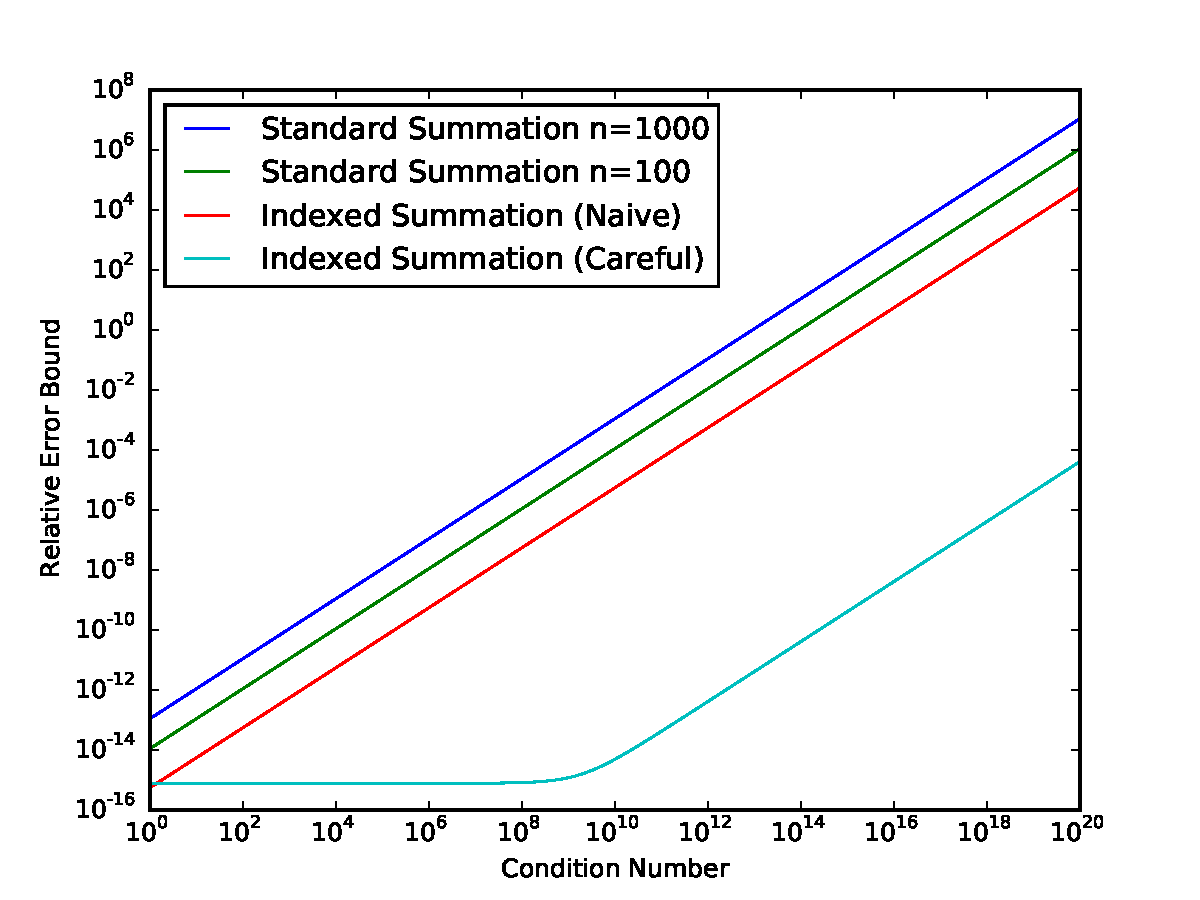
\includegraphics[width=\textwidth]{plots/errorcomparison.pdf}
\caption{Relative error bounds in calculating $|\sum \limits_{k = 0}^{n - 1} x_k|$ for different condition numbers (which we define as $\frac{n \cdot \max |x_k)}{|\sum \limits_{k = 0}^{n - 1} x_k|}$) of the sum. It is assumed that we sum using \texttt{double}, $K = 3$, and $W = 40$. ``Indexed Summation (Careful)'' corresponds to \eqref{eq:errorapproxdup}. ``Indexed Summation (Naive)'' corresponds to \eqref{eq:baderrorapproxdup}. ``Standard Summation'' corresponds to \eqref{eq:naiveerrorapproxdup} and due to a dependence on $n$ multiple error bounds are shown.}
\label{fig:conversionmotivation}
\end{center}
\end{figure}

    Consider a $K$-fold indexed type $Y$ of index $I$.
    As each value ${\mathcal{Y}_j}_P$ in a primary field ${Y_j}_P$ is represented by an offset from $1.5  \epsilon^{-1}  2^{a_{I + j}}$ and ${Y_j}_P \in (\epsilon^{-1}  2^{a_{I + j}}, 2  \epsilon^{-1}  2^{a_{I + j}})$, ${\mathcal{Y}_j}_P$ can be expressed exactly using an unnormalized floating point number ${\mathcal{Y}'_P}_j$ with an exponent of $a_{I + j} + p - 1$.
    As each carry field ${Y_j}_C$ is a count of renormalization adjustments later scaled by $0.25  \epsilon^{-1}  2^{a_{I + j}}$, ${\mathcal{Y}_j}_C$ can be expressed exactly using an unnormalized floating point number ${\mathcal{Y}'_j}_C$ with an exponent of $a_{I + j} + 2  p - 3$.

    For all $k < j$, $\exp({\mathcal{Y}'_k}_P) > \exp({\mathcal{Y}'_j}_P)$ and $\exp({\mathcal{Y}'_k}_C) > \exp({\mathcal{Y}'_j}_C)$ because $a_{I + k} > a_{I + j}$.

    Note that
    \begin{equation*}
      \exp({\mathcal{Y}'_j}_C) = a_{I + j} + 2  p - 3
    \end{equation*}

    and

    \begin{equation*}
      \exp({\mathcal{Y}'_{j - 1}}_P) = a_{I + j - 1} + p - 1 = a_{I + j} + W + p - 1
    \end{equation*}

    Therefore $\exp({\mathcal{Y}'_j}_C) > \exp({\mathcal{Y}'_{j - 1}}_P)$ using $W < p - 2$.

    Note that

    \begin{equation*}
      \exp({\mathcal{Y}'_{j - 2}}_P) = a_{I + j - 1} + p - 1 = a_{I + j} + 2 W + p - 1
    \end{equation*}

    Therefore $\exp({\mathcal{Y}'_j}_C) < \exp({\mathcal{Y}'_{j - 2}}_P)$ using $2  W > p + 1$.

    Combining the above inequalities, we see that the exponents of all the ${\mathcal{Y}'_j}_P$ and ${\mathcal{Y}'_j}_C$ are distinct and can be sorted as follows:

    \begin{alignat*}{5}
    \exp({\mathcal{Y}'_0}_C) &> \exp({\mathcal{Y}'_1}_C) &&> \exp({\mathcal{Y}'_0}_P) &&> \exp({\mathcal{Y}'_2}_C) &&> \exp({\mathcal{Y}'_1}_P) &&> ... \\
    ... &> \exp({\mathcal{Y}'_j}_C) &&> \exp({\mathcal{Y}'_{j - 1}}_P) &&> \exp({\mathcal{Y}'_{j + 1}}_C) &&> \exp({\mathcal{Y}'_j}_P) &&> ... \\
    ... &> \exp({\mathcal{Y}'_{K - 2}}_C) &&> \exp({\mathcal{Y}'_{K - 3}}_P) &&> \exp({\mathcal{Y}'_{K - 1}}_C) &&> \exp({\mathcal{Y}'_{K - 2}}_P) &&> \exp({\mathcal{Y}'_{K - 1}}_P)
    \end{alignat*}


    These unnormalized floating point numbers may, for convenience of notation, be referred to in decreasing order of unnormalized exponent as $\gamma'_0, ..., \gamma'_{2  K - 1}$.

    We have just shown that
    \begin{equation}
      \exp(\gamma_0') > ... > \exp(\gamma_{2  K - 1}')
      \label{eq:gammadecreases}
    \end{equation}

    $\gamma_k$ denotes the normalized representations of the $\gamma'_k$, and it should be noted that $\gamma_k = \gamma'_k$ as real numbers and that $\exp(\gamma_k) \leq \exp(\gamma'_k)$.

    It should be noted that if $\gamma_k$ is a primary field, then either $\gamma_{k + 1}$ or $\gamma_{k + 2}$ is a primary field. If $\gamma_k$ is a carry field, then either $\gamma_{k + 1}$ or $\gamma_{k + 2}$ is a carry field (with the exception of $\gamma_{2  K - 3}$, but in this case we have $\exp(\gamma_{2  K - 3}) = a_{I + K - 1} + 2  p - 3 \geq a_{I + K - 1} + p + \lceil\frac{p + 1}{2}\rceil - 1 = \exp(\gamma_{2  K - 1}) + \lceil\frac{p + 1}{2}\rceil$). Therefore, as $2  W > p + 1$, for all $k \in \{0, ..., 2  K - 1\}$
    \begin{equation}
      \exp(\gamma_k') \geq \exp(\gamma_{k + 2}') + W \geq \exp(\gamma_{k + 2}') + \left\lceil\frac{p + 1}{2}\right\rceil
      \label{eq:gammadecreasesfast}
    \end{equation}

    It should be noted that the ${\mathcal{Y}'_j}_P$ and the ${\mathcal{Y}'_j}_C$ can be expressed exactly using floating point types of the same precision as ${Y_j}_P$ and ${Y_j}_C$ (except in the case of overflow, in which a scaled version may be obtained), and such exact floating point representations can be obtained using  \eqref{eq:pri} and  \eqref{eq:car}.

    Now that we know how to obtain sorted, possibly scaled, fields in order of decreasing unnormalized exponent, we explain how to sum them while avoiding overflow. We will refer to the floating point type that we use to hold the sum during computation as the \textbf{intermediate} floating point type. Such a type must have at least as much precision and exponent range as the original floating point type.

    Notice that $|\gamma'_0| = |{\mathcal{Y}'_0}_C| < 2 \cdot 2^{\exp({\mathcal{Y}'_0}_C)} = 2 \cdot 2^{e_{\max} + 1 - W + 2  p - 3}$ and $\exp(\gamma'_0) > ... > \exp(\gamma'_{2  K - 1})$.  Therefore $|\gamma'_k| \leq 2^{e_{\max} - W + 2  p - 1 - k}$. The absolute value represented by an indexed type can therefore be bounded by

    \begin{equation}
      \label{eq:maxindexedvalue}
      \sum\limits_{k = 0}^{2  K - 1} |\gamma_k| < \sum\limits_{k = 0}^{2  K - 1} 2^{e_{\max} - W + 2  p - 1 - k} < \sum\limits_{k = 0}^{\infty} 2^{e_{\max} - W + 2  p - 1 - k} = 2^{e_{\max} - W + 2  p}
    \end{equation}

    If the intermediate floating point type has a maximum exponent greater than or equal to $e_{\max} - W + 2  p - 1$, then no special cases to guard against overflow are needed.

    Algorithm \ref{alg:conv2float} represents a conversion routine in such a case.

    \begin{samepage}
    \begin{alg}
      Convert $K$-fold indexed type $Y$ of index $I$ to floating point $x$. Here, $z$ is a floating point type with at least the original precision and maximum exponent $E_{\max}$ greater than $e_{\max} - W + 2  p$
      \begin{algorithmic}[1]
        \Function{ConvertIndexedToFloat}{K, x, Y}
          \State $z = {\mathcal{Y}_0}_C$
          \For{$j = 1 \To K - 1$}
            \State $z = z + {\mathcal{Y}_j}_C$
            \State $z = z + {\mathcal{Y}_{j - 1}}_P$
          \EndFor
          \State $z = z + {\mathcal{Y}_{K - 1}}_P$
          \State $x = z$ \label{alg:conv2float:conv}
        \EndFunction
      \end{algorithmic}
      \label{alg:conv2float}
    \end{alg}
    \end{samepage}

    Note that an overflow situation in Algorithm \ref{alg:conv2float} is reproducible as the fields in $Y$ are reproducible. $z$ is deterministically computed from the fields of $Y$, and the condition that $z$ overflows when being converted back to the original floating point type in line \ref{alg:conv2float:conv} is reproducible.

    If an intermediate floating point type with exponent greater than or equal to $e_{\max} - W + 2  p - 1$ is not available, the $\gamma_k$ must be scaled down by some factor during addition and the sum scaled back up when subsequent additions can no longer effect an overflow situation.

    If the scaled sum is to overflow, then its unscaled value will be greater than or equal to $2 \cdot 2^{e_{\max}}$ and it will overflow regardless of the values of any ${\mathcal{Y}_j}_P$ or ${\mathcal{Y}_j}_C$ with $|{\mathcal{Y}_j}_P| < 0.5 \cdot 2^{-\rho} 2^{e_{\max}}$ or $|{\mathcal{Y}_j}_C| < 0.5 \cdot 2^{-\rho}2^{e_{\max}}$ (where $\rho$ is the intermediate floating point type's precision). If the floating point sum has exponent greater than or equal to $e_{\max}$ these numbers are not large enough to have any effect when added to the sum. If the sum has exponent less than $e_{\max}$, then additions of these numbers cannot cause the exponent of the sum to exceed $e_{\max}$ for similar reasons.

    As the maximum absolute value of the true sum is strictly smaller than $2^{e_{\max} - W + 2  p}$, a sufficient scaling factor is $2^{2  p - W - 2}$, meaning that the maximum absolute value of the true scaled sum is strictly smaller $2 \cdot 2^{e_{\max} - 1}$ (and since it will be shown later that the computed sum is accurate to within a small factor of the true sum, the computed sum will stay strictly smaller than $2 \cdot 2^{e_{\max}}$ and will not overflow.)

  When $\exp(\gamma'_k) < e_{\max} - \rho - 1$, the sum may be scaled back up and the remaining numbers added without scaling. Notice that no overflow can occur during addition in this algorithm. If an overflow is to occur, it will happen only when scaling back up. As the fields in the indexed type are reproducible, such an overflow condition is reproducible.

    If the sum is not going to overflow, then the smaller $y'_k$ must be added as unscaled numbers to avoid underflow.

    Algorithm \ref{alg:conv2floatoverflow} represents a conversion routine in such a case.

    \begin{samepage}
    \begin{alg}
      Convert a $K$-fold indexed type $Y$ of index $I$ to floating point $x$. Here, $z$ is a floating point number with precision $\rho > p$
      \begin{algorithmic}[1]
        \Function{ConvertIndexedToFloat}{K, x, Y}
          \State $j = 1$
          \While{$j \leq 2 K$ and $\exp(\gamma_j) \geq e_{\max} - \rho - 1$}
            \State $z = z + (\gamma_j / 2^{2 p - W - 2})$
            \State $j = j + 1$
          \EndWhile
          \State $z = z \cdot 2^{2 p - W - 2}$
          \While{$j \leq 2 K$}
            \State $z = z + \gamma_j$
            \State $j = j + 1$
          \EndWhile
          \State $x = z$
        \EndFunction
      \end{algorithmic}
      \label{alg:conv2floatoverflow}
    \end{alg}
    \end{samepage}

    If an indexed type is composed of \texttt{float}, then \texttt{double} provides sufficient precision and exponent to use as an intermediate type and Algorithm \ref{alg:conv2float} may be used to convert to a floating point number.
    However, if an indexed type is composed of \texttt{double}, many machines may not have any higher precision available. We therefore perform the sum using \texttt{double} as an intermediate type. As this does not extend the exponent range we must use Algorithm \ref{alg:conv2floatoverflow} for the conversion.

  \subsection{Error Bound}
    \label{sec:primitiveops_error}

    We first state and prove Theorem \ref{thm:mysortsum}, as it is critical in the error analysis of the algorithm. It should be noted that Theorem \ref{thm:mysortsum} is similar to that of Theorem 1 from \cite{sortsum}, but requires less intermediate precision by exploiting additional structure of the input data.

    It is possible that future implementors may make modifications to the indexed type (adding multiple carry fields, changing the binning scheme, etc.) such that the summation of its fields cannot be reordered to satisfy the assumptions of Theorem \ref{thm:mysortsum}. In such an event, $\cite{sortsum}$ provides more general ways to sum the fields while still maintaining accuracy.
      \begin{samepage}
    \begin{thm}
      Given $n$ floating point numbers $f_0, ..., f_{n - 1}$ for which there exists (possibly unnormalized) floating point numbers $f'_0, ..., f'_{n - 1}$ of the same precision such that
      \begin{enumerate}
        \item $f_k = f'_k$ for all $k \in \{0, ..., n - 1\}$
        \item $\exp(f'_0) > ... > \exp(f'_{n - 1})$
        \item $\exp(f'_k) \geq \exp(f'_{k + 2}) + \lceil\frac{p + 1}{2}\rceil$ for all $k \in \{0, ..., n - 3\}$
      \end{enumerate}
      \label{thm:mysortsum}
      Let $S_0 = \overline{S_0} = f_0$, $S_k = S_{k - 1} + f_k$, and $\overline{S_k} = \fl(\overline{S_{k - 1}} + f_k)$ so that $S_{n - 1} = \sum \limits_{k = 0}^{n - 1} f_k$.
      Then we have
      \begin{equation*}
        \left|S_{n - 1} - \overline{S_{n - 1}}\right| < \frac{7\epsilon}{1 - 6\sqrt\epsilon}|S_{n - 1}| \approx 7 \epsilon |S_{n - 1}|
      \end{equation*}
    \end{thm}
    \end{samepage}

    \begin{proof}

      Throughout the proof, let $f_k = 0$ if $k > n - 1$ so that $S_{\infty} = S_{n - 1}$ and $\overline{S_{\infty}} = \overline{S_{n - 1}}$.

      Let $m$ be the location of the first error such that $S_{m - 1} = \overline{S_{m - 1}}$ and $S_{m} \neq \overline{S_{m}}$.

      If no such $m$ exists then the computed sum is exact ($S_{n - 1} = \overline{S_{n - 1}}$) and we are done.

      If such an $m$ exists, then because $\exp(f_0') > ... > \exp(f_m')$, $f_0, ..., f_m \in \ulp(f_m')\Z$. Thus, $S_m \in \ulp(f_m')\Z$.

      We now show $|S_m| > 2 \cdot 2^{\exp(f_m')}$. Assume for contradiction that $|S_m| \leq 2 \cdot 2^{\exp(f_m')}$. Because $S_m \in \ulp(f_m')\Z$, this would imply that $S_m$ is representable as a floating point number, a contradiction as $\overline{S_m} \neq S_m$. Therefore, we have
      \begin{equation}
        |S_m| > 2 \cdot 2^{\exp(f_m')}
        \label{eq:smbound}
      \end{equation}

      Because $\exp(f_m') > \exp(f_{m + 1}')$,
      \begin{equation}
        |f_{m + 1}| < 2\cdot2^{\exp(f_m' - 1)} = 2^{\exp(f_m')}
        \label{eq:smpbound}
      \end{equation}

      Because $\exp(f_m') \geq \exp(f_{m + 2}') + \lceil\frac{p + 1}{2}\rceil$ and $\exp(f_0') > ... > \exp(f_{n - 1}')$,
      \begin{align}
        \bigl|\sum \limits_{k = m + 2}^{n - 1} f_k\bigr| &\leq \sum \limits_{k = m + 2}^{n - 1} |f_k| < \sum \limits_{k = m + 2}^{n - 1} 2 \cdot 2^{\exp(f_k')} \leq \sum \limits_{k = m + 2}^{n - 1} 2 \cdot 2^{\exp(f_m') - \left\lceil\frac{p + 1}{2}\right\rceil - (m + 2 - k)} \nonumber \\
        &< \sum \limits_{k = 0}^{\infty} \left(2 \sqrt{\epsilon}\right)2^{\exp(f_m') - k} = \left(4\sqrt\epsilon\right)2^{\exp(f_m')}
        \label{eq:smppbound}
      \end{align}

      We can combine  \eqref{eq:smpbound} and \eqref{eq:smppbound} to obtain
      \begin{equation}
        \bigl|\sum\limits_{k = m + 1}^{n - 1} f_k\bigr| \leq \sum\limits_{k = m + 1}^{n - 1} |f_k| < 2^{\exp{f_m'}} + \left(4 \sqrt{\epsilon}\right) 2^{\exp(f_m')} = \left(1 + 4 \sqrt\epsilon \right)2^{\exp(f_m')}
        \label{eq:smsbound}
      \end{equation}

      By  \eqref{eq:smbound} and \eqref{eq:smsbound},
      \begin{align}
        |S_{n-1}| & = \bigl|\sum\limits_{k = 0}^{n - 1} f_k\bigr| \geq \bigl|\sum\limits_{k = 0}^{m} f_k\bigr| - \bigl|\sum\limits_{k = m + 1}^{n - 1} f_k\bigr| = |S_m| - \bigl|\sum\limits_{k = m + 1}^{n - 1} f_k\bigr| \nonumber \\
        & \geq 2 \cdot 2^{\exp(f_{m}')} - \left(1 + 4 \sqrt\epsilon\right) 2^{\exp(f_m')} = \left(1 - 4 \sqrt\epsilon\right) 2^{\exp(f_m')}
        \label{eq:sbound}
      \end{align}

      By  \eqref{eq:sbound} and \eqref{eq:smppbound},
      \begin{equation}
        \bigl|\sum \limits_{k = m + 2}^{n - 1} f_k\bigr| < \left(4 \sqrt{\epsilon}\right) 2^{\exp(f_m')} \leq \frac{4 \sqrt\epsilon}{1 - 4  \sqrt\epsilon}\bigl|\sum\limits_{k = 0}^{n - 1}f_k\bigr|
        \label{eq:smpprelsbound}
      \end{equation}

      By  \eqref{eq:sbound} and \eqref{eq:smsbound},
      \begin{equation}
        \bigl|\sum\limits_{k = m + 1}^{n - 1}f_k\bigr| \leq \sum\limits_{k = m + 1}^{n - 1}|f_k| \leq \left(1 + 4  \sqrt\epsilon\right)2^{\exp(f_m')}\leq \frac{1 + 4  \sqrt\epsilon}{1 - 4  \sqrt\epsilon}\bigl|\sum\limits_{k = 0}^{n - 1}f_k\bigr|
        \label{eq:smsrelsbound}
      \end{equation}

      And by \eqref{eq:sbound} and \eqref{eq:smsrelsbound},
      \begin{equation}
        |S_m| \leq \bigl|\sum\limits_{k = 0}^{n - 1}f_k\bigr| + \bigl|\sum\limits_{k = m + 1}^{n - 1} f_k\bigr| \leq \left(1 + \frac{1 + 4  \sqrt\epsilon}{1 - 4  \sqrt\epsilon}\right)\bigl|\sum\limits_{k = 0}^{n - 1}f_k\bigr| \leq \frac{2}{1 - 4  \sqrt\epsilon}\bigl|\sum\limits_{k = 0}^{n - 1}f_k\bigr|
        \label{eq:smrelsbound}
      \end{equation}

      By definition, $\overline{S_{m+4}}$ is the computed sum of
      $\overline{S_m}$, $f_{m+1}, \ldots, f_{m+4}$ using the standard recursive summation technique.
      According to \cite[Equation 1.2, 2.4]{higham}
      \begin{align*}
          \bigl|\overline{S_m} + \sum_{k=m+1}^{m+4}f_k - \overline{S_{m+4}}\bigr|
          & \leq \frac{4\epsilon}{1-4\epsilon} \left|\overline{S_m} + f_{m+1}\right| + \frac{3\epsilon}{1-3\epsilon} \sum_{k=m+2}^{m+4}|f_k| \\
          & \leq \frac{4\epsilon}{1-4\epsilon} \bigl(\left|\overline{S_m} - S_m\right| + |S_m + f_{m+1}|\bigr)
              + \frac{3\epsilon}{1-3\epsilon} \sum_{k=m+2}^{n-1}|f_k|.
      \end{align*}
      Since $S_{n-1} = S_m + f_{m+1} + \sum_{k=m+2}^{n-1} f_k$, we have
      \begin{equation*}
          |S_m + f_{m+1}|
          = \bigl|S_{n-1} - \sum_{k=m+2}^{n-1}f_k\bigr|
          \leq |S_{n-1}| + \sum_{k=m+2}^{n-1} |f_k|
      \end{equation*}
      Therefore
      \begin{equation*}
          \bigl|\overline{S_m} + \sum_{k=m+1}^{m+4}f_k - \overline{S_{m+4}}\bigr|
          \leq \frac{4\epsilon}{1-4\epsilon} \left|S_m - \overline{S_m}\right|
          + \frac{4\epsilon}{1-4\epsilon} |S_{n-1}|
          + \frac{7\epsilon}{1-4\epsilon} \sum_{k=m+2}^{n-1}|f_k|.
      \end{equation*}
      Using the Triangle Inequality we have
      \begin{align*}
      \left|S_{m+4} - \overline{S_{m+4}}\right|
          & = \bigl|S_m + \sum_{k=m+1}^{m+4}f_k - \overline{S_{m+4}}\bigr|
          \leq \left|S_m - \overline{S_m} \right| + \bigl|\overline{S_m} + \sum_{k=m+1}^{m+4}f_k - \overline{S_{m+4}} \bigr| \\
          & \leq \left(1 + \frac{4\epsilon}{1-4\epsilon}\right) \left|S_m - \overline{S_m}\right| + \frac{4\epsilon}{1-4\epsilon} |S_{n-1}|
                  + \frac{7\epsilon}{1-4\epsilon} \sum_{k=m+2}^{n-1}|f_k| \\
          & \leq \frac{1}{1-4\epsilon} \epsilon |S_m| + \frac{4\epsilon}{1-4\epsilon} |S_{n-1}|
                  + \frac{7\epsilon}{1-4\epsilon} \sum_{k=m+2}^{n-1}|f_k| \\
          & \leq \frac{\epsilon}{1-4\epsilon} \left(|S_m| + 4 |S_{n-1}|
                  + 7 \sum_{k=m+2}^{n-1}|f_k|\right).
      \end{align*}
      and by \eqref{eq:smrelsbound} and \eqref{eq:smpprelsbound},
      \begin{align}
      \left|S_{m+4} - \overline{S_{m+4}}\right|
          & \leq \frac{\epsilon}{1-4\epsilon}
              \left(
                  \frac{2}{1-4\sqrt{\epsilon}} |S_{n-1}|
                  + 4 |S_{n-1}|
                  + 7 \frac{4\sqrt{\epsilon}}{1-4\sqrt{\epsilon}} |S_{n-1}|
              \right) \nonumber \\
          & \leq \frac{\epsilon}{1-4\epsilon} \left(\frac{6+12\sqrt{\epsilon}}{1-4\sqrt{\epsilon}} |S_{n-1}|\right)
              = \frac{6\epsilon }{(1-2\sqrt{\epsilon})(1-4\sqrt{\epsilon})} |S_{n-1}| \nonumber \\
          & < \frac{6\epsilon}{1-6\sqrt{\epsilon}} |S_{n-1}|
          \label{eq:smfiveerror}
      \end{align}

      Notice that
      \begin{equation*}
        \exp(f_m') \geq \exp(f_{m + 2}') + \left\lceil\frac{p+ 1}{2}\right\rceil \geq \exp(f_{m + 4}') + 2  \left\lceil\frac{p + 1}{2}\right\rceil > \exp(f_{m + 5}')+ 2  \left\lceil\frac{p+ 1}{2}\right\rceil
      \end{equation*}
      Therefore,
      \begin{equation}
        \exp(f_m') \geq \exp(f_{m + 5}') + p + 2
        \label{eq:fmfiveexp}
      \end{equation}

      Because $\exp(f_0') > ... > \exp(f_{n - 1}')$, \eqref{eq:fmfiveexp} yields
      \begin{equation}
        \bigl|\sum\limits_{k = m + 5}^{n - 1} f_k\bigr| \leq \sum\limits_{k = m + 5}^{n - 1} |f_k| < \sum\limits_{k = m + 5}^{n - 1} 2 \cdot 2^{\exp(f_m') - p - 2 - (k - (m + 5))} < \sum\limits_{k = 0}^{\infty} 2^{\exp(f_m') - p - 1 - k} = \epsilon 2^{\exp(f_m')}
        \label{eq:boundfmfivesum}
      \end{equation}

      Using \eqref{eq:sbound} and \eqref{eq:boundfmfivesum},
      \begin{equation}
        \bigl|\sum\limits_{k = m + 5}^{n - 1} f_k\bigr| \leq \sum\limits_{k = m + 5}^{n - 1} |f_k| < \frac{\epsilon}{1 - 4  \sqrt\epsilon}|S_{n - 1}|
        \label{eq:relsboundfmfivesum}
      \end{equation}

      By \eqref{eq:smfiveerror} and \eqref{eq:relsboundfmfivesum}
      \begin{align}
        \left|S_{n-1} - \overline{S_{m+4}}\right|
        & \leq |S_{n-1} - S_{m+4}| + \left|S_{m+4} - \overline{S_{m+4}}\right| \nonumber \\
        & \leq \bigl|\sum_{k=m+4}^{n-1} f_k\bigr| + \frac{6\epsilon}{1-6\sqrt{\epsilon}} |S_{n-1}| \nonumber \\
        & \leq \frac{\epsilon}{1 - 4 \sqrt\epsilon}|S_{n-1}| + \frac{6\epsilon}{1-6\sqrt{\epsilon}} |S_{n-1}| \nonumber \\
        & <  \frac{7\epsilon}{1-6\sqrt{\epsilon}} |S_{n-1}|.
        \label{eq:smfiveerror-1}
      \end{align}

      When combined with \eqref{eq:sbound} gives
      \begin{align*}
        \left|\overline{S_{m+4}}\right|
        & \geq \left(1-\frac{7 \epsilon}{1-6\sqrt{\epsilon}}\right) |S_{n-1}| \\
        & > \left(1-\frac{7 \epsilon}{1-6\sqrt{\epsilon}}\right) \left(1-4\sqrt{\epsilon}\right) 2^{\exp(f'_m)} \\
        & > \left(1-4\sqrt{\epsilon} - \frac{7 \epsilon \left(1-4\sqrt{\epsilon}\right)}{1-6\sqrt{\epsilon}}\right) 2^{\exp(f'_m)}
      \end{align*}

      which, assuming $\epsilon << 1$, can be simplified to
      \begin{equation}
        \left|\overline{S_{m + 4}}\right| > 2^{\exp(f_m') - 1}
        \label{eq:minsmfoursimple}
      \end{equation}

      Using  \eqref{eq:fmfiveexp}, for all $k \geq m + 5$ we have

      \begin{equation}
        |f_k| < 2 \cdot 2^{\exp(f_k')} \leq 2 \cdot 2^{\exp(f_m) - p - 2} = \epsilon \cdot 2^{\exp(f_m') - 1}
        \label{eq:maxfmfive}
      \end{equation}

      And by \eqref{eq:maxfmfive} and \eqref{eq:minsmfoursimple}, all additions after $f_{m + 4}$ have no effect and we have $\overline{S_{n-1}} = \overline{S_{m+4}}$.
      This, together with \eqref{eq:smfiveerror-1}, implies
      \begin{equation*}
        \left|S_{n-1} - \overline{S_{n-1}}\right| \leq \frac{7\epsilon}{1-6\sqrt{\epsilon}} |S_{n-1}|
      \end{equation*}
      The proof is complete.
    \end{proof}

    Consider the $K$-fold indexed sum $Y$ of floating point numbers $x_0, ..., x_{n - 1}$. We denote the true sum $\sum \limits_{k = 0}^{n - 1} x_k$ by $T$, the true value of the indexed sum as obtained using  \eqref{eq:indexedvalue} by $\mathcal{Y}$, and the floating point approximation of $\mathcal{Y}$ obtained using an appropriate algorithm from Section \ref{sec:primitiveops_convert} by $\overline{\mathcal{Y}}$.

    \cite{repsum} discusses the absolute error $|T - \mathcal{Y}|$ but does not give a method to construct $\overline{\mathcal{Y}}$ and therefore no error bound ($|T - \overline{\mathcal{Y}}|$) on the final floating point answer was given. Here we extend the error bound of \cite{repsum} all the way to the final return value of the algorithm.

    It has been shown in \cite{repsum} that

    \begin{equation}
      \label{eq:repboundnaive}
      |T - \mathcal{Y}| < n  2^{W  (1 - K) - 1}\max|x_k|
    \end{equation}

    However, this bound does not consider underflow. By  \eqref{eq:droundunderflow}, a small modification yields a bound that considers underflow

    \begin{equation}
      \label{eq:repbound}
      |T - \mathcal{Y}| < n \cdot \max\bigl(2^{W  (1 - K) - 1} \max|x_k|, 2^{e_{\min} - 1}\bigr)
    \end{equation}

    By  \eqref{eq:gammadecreases} and \eqref{eq:gammadecreasesfast}, Theorem \ref{thm:mysortsum} applies to yield

    \begin{equation*}
      \left|\mathcal{Y} - \overline{\mathcal{Y}}\right| < \frac{7\epsilon}{1 - 6\sqrt\epsilon}|\mathcal{Y}|
    \end{equation*}

    By the triangle inequality

    \begin{equation*}
      |\mathcal{Y}| \leq |T| + |T - \mathcal{Y}| < n \cdot \max\bigl(2^{W  (1 - K) - 1}  \max|x_k|, 2^{e_{\min} - 1}\bigr) + |T|
    \end{equation*}

    The above results can be used to obtain  \eqref{eq:error}, the absolute error of the floating point approximation of an indexed sum $|T - \overline{\mathcal{Y}}|$.

    \begin{align}
      \left|T - \overline{\mathcal{Y}}\right| &\leq |T - \mathcal{Y}| + \left|\mathcal{Y} - \overline{\mathcal{Y}}\right| \nonumber \\
      &< n \cdot \max\bigl(2^{W  (1 - K) - 1}  \max|x_k|, 2^{e_{\min} - 1}\bigr) + \frac{7\epsilon}{1 - 6\sqrt\epsilon} |\mathcal{Y}| \nonumber \\
      &< n \cdot \max\bigl(2^{W  (1 - K) - 1}  \max|x_k|, 2^{e_{\min} - 1}\bigr) \nonumber \\
      &+ \frac{7\epsilon}{1 - 6\sqrt\epsilon} \Bigl(n \cdot \max\bigl(2^{W  (1 - K) - 1}  \max|x_k|, 2^{e_{\min} - 1}\bigr) + |T|\Bigr) \nonumber \\
      &< \left(1 + \frac{7\epsilon}{1 - 6\sqrt\epsilon}\right) \Bigl(n \cdot \max\bigl(2^{W (1 - K) - 1} \max|x_k|, 2^{e_{\min} - 1}\bigr)\Bigr) + \frac{7\epsilon}{1 - 6\sqrt\epsilon} |T|
      \label{eq:error}
    \end{align}

    Equation \eqref{eq:error} can be approximated as \eqref{eq:errorapprox}.

    \begin{align}
      \left|T - \overline{\mathcal{Y}}\right| &< \left(1 + \frac{7\epsilon}{1 - 6\sqrt\epsilon}\right) \Bigl(n \cdot \max\bigl(2^{W (1 - K) - 1} \max|x_k|, 2^{e_{\min} - 1}\bigr)\Bigr) + \frac{7\epsilon}{1 - 6\sqrt\epsilon} |T| \nonumber \\
    &\approx n 2^{W  (1 - K) - 1} \max|x_k| + 7  \epsilon |T|
      \label{eq:errorapprox}
    \end{align}

    A perhaps more useful mathematical construction is the error expressed relative to the result $\overline{\mathcal{Y}}$, and not the theoretical sum $T$. Again by the triangle inequality,

    \begin{equation*}
      |\mathcal{Y}| \leq \left|\overline{\mathcal{Y}}\right| + \left|\mathcal{Y} - \overline{\mathcal{Y}}\right|
    \end{equation*}

    Applying the bound on $|\mathcal{Y} - \overline{\mathcal{Y}}|$ yields

    \begin{equation*}
      |\mathcal{Y}| < \left|\overline{\mathcal{Y}}\right| + \frac{7\epsilon}{1 - 6\sqrt\epsilon}|\mathcal{Y}|
    \end{equation*}

    After simplification,

    \begin{align*}
      |\mathcal{Y}| &< \left(\frac{1}{1 - \frac{7\epsilon}{1 - 6\sqrt\epsilon}}\right)  \left|\overline{\mathcal{Y}}\right| \nonumber \\
      &< \frac{1 - 6 \sqrt\epsilon}{1 - 6 \sqrt \epsilon - 7\epsilon}  \left|\overline{\mathcal{Y}}\right|
    \end{align*}

    The above results can be used to obtain  \eqref{eq:error2}, the absolute error of the floating point approximation of an indexed sum $|T - \overline{\mathcal{Y}}|$.

    \begin{align}
      \left|T - \overline{\mathcal{Y}}\right| &\leq |T - \mathcal{Y}| + \left|\mathcal{Y} - \overline{\mathcal{Y}}\right| \nonumber \\
      &< n \cdot \max\bigl(2^{W  (1 - K) - 1}  \max|x_k|, 2^{e_{\min} - 1}\bigr) + \frac{7\epsilon}{1 - 6\sqrt\epsilon}|\mathcal{Y}| \nonumber \\
      &< n \cdot \max\bigl(2^{W  (1 - K) - 1}  \max|x_k|, 2^{e_{\min} - 1}\bigr) + \frac{7\epsilon}{1 - 6\sqrt\epsilon}\left(\frac{1 - 6 \sqrt\epsilon}{1 - 6 \sqrt \epsilon - 7\epsilon}\left|\overline{\mathcal{Y}}\right|\right) \nonumber \\
      &< n \cdot \max\bigl(2^{W  (1 - K) - 1}  \max|x_k|, 2^{e_{\min} - 1}\bigr) + \frac{7\epsilon}{1 - 6 \sqrt \epsilon - 7\epsilon}\left|\overline{\mathcal{Y}}\right|
      \label{eq:error2}
    \end{align}

    Equation \eqref{eq:error2} can be approximated as  \eqref{eq:error2approx}.

    \begin{align}
      |T - \overline{\mathcal{Y}}| &< n \cdot \max\bigl(2^{W  (1 - K) - 1}  \max|x_k|, 2^{e_{\min} - 1}\bigr) + \frac{7\epsilon}{1 - 6 \sqrt \epsilon - 7\epsilon}  \left|\overline{\mathcal{Y}}\right| \nonumber \\
      &\approx n  2^{W  (1 - K) - 1} \max|x_k|+ 7 \epsilon \left|\overline{\mathcal{Y}}\right|
      \label{eq:error2approx}
    \end{align}

    We can compare  \eqref{eq:errorapprox} to the error bound obtained if the accumulator fields were summed without extra precision. In this case, only the standard summation bound from \cite{higham} would apply and the absolute error would be bounded by

    \begin{equation*}
    n \cdot \max\bigl(2^{W  (1 - K) - 1}  \max|x_k|, 2^{e_{\min} - 1}\bigr) + \left(\frac{(2  K - 1)  \epsilon}{1 - (2  K - 1)  \epsilon}\right)  \sum\limits_0^{2  K - 1}|\gamma_k|
    \end{equation*}
    which is approximately bounded by
    \begin{equation}
    n \cdot \max|x_k| \bigl(2^{W  (1 - K) - 1} + (2  K - 1)  \epsilon\bigr)
    \label{eq:baderrorapprox}
    \end{equation}

    Which is not as tight a bound as \eqref{eq:errorapprox}, and grows linearly as the user increases $K$ in an attempt to increase accuracy.

  \subsection{Limits}
    \label{sec:primitiveops_limits}
    As discussed previously, for a $K$-fold indexed type the minimum $K$ accepted by ReproBLAS is 2. The maximum useful $K$ is $\lfloor(e_{\max} - e_{\min} + p - 1)/W\rfloor$, as this covers all of the bins.

    As discussed in \cite{repsum}, $W < p - 2$. As discussed in section \ref{sec:indexed_overflow}, $2 W > p + 1$.

    ReproBLAS uses the values $W = 40$ for indexed \texttt{double} and $W = 13$ for indexed \texttt{float}. $W$ is available as the \texttt{XIWIDTH} macro.

    As discussed in section \ref{sec:indexed_underflow_gradual}, the input is rounded at best to the nearest $2^{e_{\min} - 1}$

    As absolute value of individual quantities added to ${Y_j}_P$ are not in excess of $2^{b_{I + j}}$, a maximum of $0.25\epsilon^{-1}2^{-W}$ elements may be deposited into ${Y_j}_P$ between renormalizations, as discussed in section \ref{sec:primitiveops_renormalize}. For indexed \texttt{double} this number is $2^{11}$, whereas for indexed \texttt{float} this number is $2^9$. This number is supplied programmatically using the \texttt{XIENDURANCE} macro.

    By \eqref{eq:totalfreq}, an indexed sum is capable of representing the sum of at least $0.25\epsilon^{-1}2^{-W}  (\epsilon^{-1} - 1) \approx 2^{2  p - W - 2}$ floating point numbers. For indexed \texttt{double} this number is almost $2^{64}$, whereas for indexed \texttt{float} this number is almost $2^{33}$. This number is supplied programmatically using the \texttt{XICAPACITY} macro.

    The indexed types provided by ReproBLAS will, when used correctly, avoid intermediate overflow.

\section{Interface}
  \subsection{Section Summary}
  \subsection{Fold}
  \subsection{Complex Types}
  \subsection{Naming Conventions}
  \subsection{Build System}
\section{indexed.h}
  \subsection{Section Summary}
  \subsection{Types}
  \subsection{Functions}
    \subsubsection{xixadd}
    \subsubsection{xixiadd}
    \subsubsection{xscale}
    \subsubsection{xixiaddsq}
\section{idxdBLAS.h}
  \label{sec:idxdBLAS}
  \subsection{Section Summary}
  \subsection{Functions}
    \subsubsection{xixdot}
    \subsubsection{xixnrm2}
    \subsubsection{xixgemv}
    \subsubsection{xixgemm}
  \subsection{Optimization}
    Due to the proportion of time spent in the deposit routine, optimization of the deposit routine was prioritized. In the event that multiple $x$ need to be added to $Y$, the deposit routine can be vectorized by accumulating the $x$ in multiple copies of $Y$. The number of copies of $Y$ to make, $c$, and the number of unrolled loop iterations, $u$ are tuning parameters.
\section{repBLAS.h}
  \subsection{Section Summary}
\section{idxdMPI.h}
  \subsection{Section Summary}
  \subsection{Types}
  \subsection{Functions}
    \subsubsection{XIXIREDUCE}
\section{Applications}
  \subsection{Section Summary}
  \subsection{Parallel Reproducible Dot Product}
  \subsection{Parallel Reproducible Vector Norm}
  \subsection{Parallel Reproducible Matrix-Vector Multiply}
  \subsection{Parallel Reproducible Matrix-Matrix Multiply}
\begin{thebibliography}{9}
  \bibitem{repsum}
    Demmel, James, and Hong Diep Nguyen. Parallel Reproducible Summation. IEEE Transactions on Computers, 2014.
  \bibitem{ieee754}
    IEEE Standard for Floating-Point Arithmetic, IEEE Std 754-2008 , vol., no., pp.1,70, Aug. 29 2008
  \bibitem{c89}
    ANSI/ISO 9899-1990 American National Standard for Programming Languages - C, section 6.1.2.5
  \bibitem{higham}
    Higham, Nicholas J. The accuracy of floating point summation. SIAM Journal on Scientific Computing 14, no. 4 (1993): 783-799.
  \bibitem{sortsum}
    Demmel, James W., and Yozo Hida. Accurate floating point summation. Computer Science Division, University of California, 2002.
  %\bibitem{doubledouble}
  %  Hida, Yozo, Xiaoye S. Li, and David H. Bailey. Quad-double arithmetic: Algorithms, implementation, and application. 15th IEEE Symposium on Computer Arithmetic, 2000.
\end{thebibliography}
\end{document}
